\documentclass[11pt]{article}

\usepackage{paper}
\usepackage{caption}
\usepackage{subcaption}
\usepackage{float}

\definecolor{mygreen}{rgb}{0,0.6,0}
\definecolor{mygray}{rgb}{0.5,0.5,0.5}
\definecolor{mymauve}{rgb}{0.58,0,0.82}

\lstset{ %
    language=python,
    backgroundcolor=\color{white},   % choose the background color
    basicstyle=\footnotesize,        % size of fonts used for the code
    breaklines=true,                 % automatic line breaking only at whitespace
    captionpos=b,                    % sets the caption-position to bottom
    commentstyle=\color{mygreen},    % comment style
    escapeinside={\%*}{*)},          % if you want to add LaTeX within your code
    keywordstyle=\color{blue},       % keyword style
    stringstyle=\color{mymauve},     % string literal style
    otherkeywords={np,self},
    frame=lines,
    escapeinside={(*@}{@*)},
}

\begin{document}
    \title{Variations in Stellar Metallicity}
    \author[20460785]{Thomas C. Fraser}{University of Waterloo, Waterloo, Ontario, Canada}
    \date{April 6th, 2016}
    \abstract{The metallicity and age of a star are closely related due to the composition of material left behind parent star(s). Older stars where formed when less metal was present and are expected to have lower metallicities. Does low metallicity provided an explaination as to why we have yet to observe any population III stars?}
    \section*{Introduction}
    This report aims to discuss the methods used and results obtained while conducting the stellar modeling project outlined in the final project description \cite{projectdesciption}. In summary, the purpose of the project is to build a working stellar model for main sequence stars, then modifying a particular component of the model and analyzing the effects on real astronomical observables. More specifically, this report examines the stellar model's response upon changing the metallic composition of the star. \\

    The stellar model in question is essentially a set of coupled ordinary differential equations that needs to be solved numerically in conjunction with a set of initial conditions and boundary conditions. To begin, this report will outline motivations behind why this work is important. Afterwards, the stellar model will be described in brief in order to motivate particular phenomena observed in the results of this project. The model will give the setting for the computational techniques and choices made in order to obtain solutions to this model. As will be seen, special steps were needed in order to define initial conditions as well as solve for boundary conditions. \\

    Lastly, the results will be presented and accompanied by qualitative analysis. As a case study, two stars with the same composition but drastically different surface features will be compared in order to understand the effectiveness of the model. Second, two stars with identical central temperatures but varying metallicity will be compared to examine how metallicity affects the observed surface features. Finally numerous stars at different metallicities were generated to be plotted in a main sequence and then compared with empirical luminosity-mass and radius-mass relationships. \\

    To conclude, this report will discuss some issues and limitations of the model and suggest areas for improvement, specifically in the context of modeling metallicity.

    \section*{Acknowledgments}
    This report was written individually but represents work conducted by Thomas Coolican Fraser (myself), Robert Charles Burnet, Joseph Nelson Ulmer, Tiaotiao Chen, and Tiasa Mondol (in no particular order). This body of work and code produced is the result of contributions from all group members and could not have been completed without everyone's help. I thank them immensely. In addition, I would personally like to thank Avery Broderick for the knowledge and wisdom imparted onto us. Without his guidance and expertise, this project would have been far less successful.

    \section{Motivations and Stellar Populations}
    Stars are fascinating. They are a pillar of astronomy and integral to our history as a species. There are a bounty of reasons for modeling and studying stars. But what makes studying their metallicity particularly important?
    \subsection{Metallicity}
    The metallicity of a star, denoted $Z$ is the metal mass fraction within a star \cite{textbook}. ``Metal'' meaning all elements with nuclei heavier that helium.
    \[ Z \defined \f{\rho\tsb{metal}}{\rho} \]
    Analogously, there are corresponding mass fractions for hydrogen and helium respectively $X$ and $Y$. A star with high metallicity has a large proportional of heavy nuclei. As a result of this, metallicity is closely related to the age of a star. Throughout the course of this project, there are a few simplifying assumptions made that directly pertain to the metallicity of the star. The first being that the composition is \textit{constant} throughout the star. In general one would expect the composition of the material in the star to vary as a function of radius with heavy nuclei concentrated towards the central regions of the star where they are produced via fusion. Secondly, the material in the star is taken to be purely ionized. This gives a constant mean molecular mass,
    \[ \mu\tsb{ionized} = \br{2X + \f34 Y + \f12 Z}^{-1} \]
    This approximation works fine at high temperatures where the atoms are more likely to be ionized; albeit a poor approximation when the temperature decreases near the surface. Finally, the mass fractions are required to sum to unity, $X + Y + Z = 1$, thus modifying $Z$ necessarily means modifying $X$ and/or $Y$ as well. The stellar model described in section \ref{sec:modelbasics} depends more heavily on the hydrogen mass fraction $X$ (due to the energy production terms $\ep$). With this in mind, isolating the effects of changing $Z$ will be easier if throughout this report and in all the stars generated, the hydrogen mass fraction is taken to be the constant solar value $X = X_\odot = 0.73$.
    \subsection{Stellar Populations}
    Individual stars can be categorized into 3 populations. These populations are characterized by their metallicity. Population I stars are the highest metallicity stars observed with metallicities $Z \geq 0.01$. Our sun is an example of a population I star. These stars are heavy in metals because they were created from the remnants of dead older stars. As such they are relatively young stars with ages ranging from $\SI{1}{\giga\yr}$ to $\SI{10}{\giga\yr}$. Population II stars are an older class of stars with ages $\geq\SI{10}{\giga\yr}$. Since there was less metallic material  present during formation, they have considerably smaller metallicities $Z \leq 0.001$. The collection of stars found in the M80 globular cluster are examples of Pop. II stars. Finally and most fascinating are population III stars. These hypothetical stars would be the earliest formed stars with ages comparable to the age of the universe. They are extremely metal poor $Z \ll 1$; possibly zero metallicity $Z = 0$. \\

    As one would expect, the composition of a star is heavily related to the conditions present during formation. Different parent star histories, cluster conditions, interstellar densities, interactions with other bodies, etc. all affect the conditions of stellar formation. Therefore metallicity is not always a one-to-one relationship with the age of a star. Nonetheless, this high-level trend is the scope of this project. \\

    Studying the observables of stars generated with nearly zero metallicity allows us to determine what features to look for in order to discover population III stars. One goal of this body of work is to determine where to look for the oldest stars. The second goal is to potentially explain and motivate why we have not observed any before.
    \section{Model Basics}
    \label{sec:modelbasics}
    Before discussing the techniques and methods used to obtain solutions to the stellar model, this section aims to outline some of the basic ideas of the stellar model in question. This is done in motivation to draw specific reference to equations and strategies used to make programming decisions as well as interpret results.\\

    The model consists of 5 equations that govern the equations of stellar structure. The first being hydrostatic equilibrium,
    \[ \der{\rho}{r} = - \bs{\f{GM\rho}{r^2} + \pder{P}{T}\der{T}{r}} \br{\pder{P}{\rho}}^{-1} \eq\label{eq:hydrostaticequilibrium} \]
    Together with three distinct contributions to the pressure; respectively non-relativistic degeneracy pressure, ideal gas pressure, and radiative pressure,
    \[ P\br{\rho, T} = \f{\br{3\pi^2}^{2/3}}{5}\f{\hbar^2}{m_e}\br{\f{\rho}{m_p}}^{5/3} + \rho \f{kT}{\mu m_p} + \f13 a T^4 \eq \label{eq:partialpressures} \]
    The second being energy transport either governed by radiative transport or convective bulk motions respectively,
    \[ \der{T}{r} = - \min \bs{\f{3\kappa \rho L}{16 \pi a c T^3 r}, \br{1 - \f{1}{\ga}}\f{T}{P}\f{GM\rho}{r^2}} \eq \label{eq:energytransport} \]
    The remaining three equations being mass continuity, energy production and optical depth respectively,
    \[ \der{M}{r} = 4 \pi r^2 \rho \eq \label{eq:masscontinuity} \]
    \[ \der{L}{r} = \der{M}{r} \ep \eq \label{eq:energyproduction} \]
    \[ \der{\tau}{r} = - \kappa \rho \eq \label{eq:opticaldepth} \]
    Note that the optical depth differential equation is not solved explicitly, albeit introduced as the first of two boundary conditions. The optical depth increases as one's line-of-sight approaches the center of the star from the outside. Consequently, the surface or radius of the star $R_*$ is defined via the Eddington approximation where the optical depth reaches $2/3$ \cite{eddington}. Therefore when integrating from the center of the star outward, the surface of the star is reached when the remaining optical depth falls to $2/3$.
    \[ \tau\br{\inf} - \tau\br{R_*} = \f23 \eq \label{eq:tauboundary} \]
    As a means of approximating the remaining optical depth, the following is used,
    \[ \tau\br{\inf} - \tau\br{R_*} \defined \f{\ka \rho^2}{\abs{\dif \rho / \dif r}} \eq \label{eq:tauproxy} \]
    Using this first boundary condition \eqref{eq:tauboundary}, the radius of the star is fixed. Then the remaining boundary condition is given by the Stefan-Boltzmann law for black-body radiation,
    \[ L\br{R_*} = 4 \pi \si R_*^2 T_*^4 \eq \label{eq:lumin-boundary}\]
    It is important to note that the surface luminosity for a particular radius is decided by the energy production within the star \eqref{eq:energyproduction}. Therefore satisfying \eqref{eq:lumin-boundary} becomes a problem of picking the right initial conditions such that,
    \[ L\br{R_*} = L_* \]
    Finally, the desired initial conditions for the center of the star are,
    \[ \rho\br{0} = \rho_c \quad T\br{0} = T_c \quad M\br{0} = 0 \quad L\br{0} = 0 \eq \label{eq:desiredinitialconditions} \]
    However careful inspection of \eqref{eq:hydrostaticequilibrium}, \eqref{eq:energytransport}, \eqref{eq:masscontinuity} and \eqref{eq:energyproduction} indicates the initial conditions \eqref{eq:desiredinitialconditions} lead to several division by zero issues. To mitigate this, the initial conditions are taken at a very small (compared to the system) radius ($r_0 = \SI{1}{\m}$) where,
    \[ \rho\br{r_0} = \rho_c \quad T\br{r_0} = T_c \quad M\br{r_0} = \f{4\pi}{3}r_0^3 \rho_c \quad L\br{r_0} = M\br{r_0} \ep\br{r_0} \eq \label{eq:initialconditions} \]
    Where $\rho_c$ and $T_c$ are at taken as free parameters with $\rho_c$ eventually determined by the luminosity boundary condition \eqref{eq:lumin-boundary}.
    \subsection{Opacity}
    \label{sec:opacity}
    When examining the stellar model with metallicity in mind, the most important components are the opacity sources. In this model we are considering 3 distinct sources of opacity. First, electron scattering due to electrons deviating from their original trajectory by interacting with positively charged nuclei, emitting radiation.
    \[ \ka\tsb{es} = 0.02 \br{1+X}\SI{}{\m^2\per\kg} \eq \label{eq:kes}\]
    Second, opacity can be dominated by Kramer's free-free absorption when photons are absorbed by an ion and then re-emitted.
    \[ \ka\tsb{ff} = \SI{1e24}{}\br{Z + 0.0001}\rho_3^{0.7}T^{-3.5}\SI{}{\m^2\per\kg} \eq \label{eq:kff}\]
    Finally, at the surface of the star when the temperature is low enough for there to be neutral hydrogen, a hydrogen atom can capture an electron to become $\text{H}^-$ which further disrupts other electrons and contributes to the opacity near the surface.
    \[ \ka_{\text{H}^-} = \SI{2.5e-32}{}\br{Z/0.02} \rho_3^{0.5} T^9 \SI{}{\m^2\per\kg} \eq\label{eq:kh}\]
    Near the center of the star, the opacity is dominated by the maximum of $\ka\tsb{es}$ and $\ka\tsb{ff}$. Whereas near the surface, $\ka_{\text{H}^-}$ completely dominates. Therefore an appropriate combination of these three sources is given by,
    \[ \ka\br{\rho, T} = \bs{\f{1}{\ka_{\text{H}^-}} + \f{1}{\max\br{\ka\tsb{es},\ka\tsb{ff}}}}^{-1} \eq\label{eq:opacitycombo} \]
    In particular, notice that as central temperature increases, there will eventually be a point where the electron scattering opacity begins to dominate the free-free opacity due to the $T^{-3.5}$ dependence in the free-free opacity term \eqref{eq:kff}. It is expected that with increasing temperature, the central opacities will decrease up until a critical point. After this point, the radiative transport term in \eqref{eq:energytransport} will be kept larger that otherwise expected for free-free opacity. With higher opacities, it becomes harder for energy to be transported via radiation. This partially explains why a convective core dominates when the central temperatures get high enough (other effects include higher temperatures forcing the CNO cycle to be dominant in energy production and radiative pressure to be dominant at high temperatures). \\

    At the center of a star, this phenomena of increasing temperature is effectively the same as decreasing $Z$ (see \eqref{eq:kff}). One would expect that with decreasing metallicity $Z$, eventually the electron scattering opacity will begin to dominate and drive a convective core. Albeit, one would not expect the radiative pressure term to dominate as temperature is temperature is held constant when varying metallicity. This is precisely the behavior observed, as will be seen section \ref{sec:varyingmetallicity}. \\

    What happens when $Z$ becomes exactly zero? Upon naive substitution of $Z = 0$ into \eqref{eq:opacitycombo}, one sees that the total stellar opacity tends to $\kappa \ar 0$ for all radii. This seems to demand that the star be purely radiative. Furthermore, $\text{H}^-$ opacity is required to turn the outer surface convective and define the photosphere of the star. When $\kappa$ tends to zero, the optical depth boundary condition \eqref{eq:tauproxy} is ill-defined. What is the problem? \\

    It is important to realize that the $\text{H}^-$ only contributes for low temperatures at the surface of the star. In the center of the star, it doesn't contribute at all because all of the hydrogen is ionized. The center of the star will always be dominated by either the electron scattering or free-free opacity. Since the electron scattering opacity is constant and finite (for fixed $X$) and the free-free opacity has a finite minimum when $Z = 0$, the opacity still remains finite even for very, very low metallicity. However, there still exists a lower limit for $Z$ where the model is unable to resolve this conflict; there will always be a $Z$ small enough that $\text{H}^-$ opacity dominates even at the center of the star. However, quantitative tests using typical stellar parameters suggest that this effect does not manifest itself until $Z < \SI{1e-100}{}$. A quick approximation yields that the maximum number of particles in the sun is,
    \[ n = \f{M_\odot}{\ba{m_i}} < 2\f{M_\odot}{m_p} = 2 \cdot \f{\SI{1.989e30}{\kg}}{\SI{1.67e-27}{\kg}} \approx \SI{2e57}{} \]
    Which suggests that $Z = \SI{1e-100}{}$ is entire non-physical. Therefore, $Z=0$ is an edge-case of the model that is not properly supported. Therefore, the project aims to study the limit of $Z$ approaching $0$ in hopes that insights will be learned nonetheless.
    \section{Code}
    \subsection{Preface}
    Python was the programming language chosen to write all of the code for this project. This choice was made because the majority of group members had experience with Python before and alternatives such as Matlab or C++ had less support within the group. All code for this project can be found on Github at the provided reference \cite{githubcode}.
    \subsection{Methods}
    \subsubsection{Runge-Kutta-Fehlberg Method}
    \label{sec:rkf}
    In order to solve the differential equations outlined in section \ref{sec:modelbasics}, we used a 4th-5th order adaptive step-size algorithm known as the Runge-Kutta-Fehlberg (RKF) method \cite{rkf}. The finite difference coefficients were taken from the provided reference, while the main algorithm was slightly modified for the purposes of this project. The core of the algorithm lies when computing the integration error and then changing the step-size accordingly,
    \begin{lstlisting}
    def rkf(f, a, x0, tol, stop):
    (*@\centerline{\raisebox{-1pt}[0pt][0pt]{$\vdots$}}@*)
        while not stop(i,x,t):
    (*@\centerline{\raisebox{-1pt}[0pt][0pt]{$\vdots$}}@*)
            # Compute 4th/5th order Runge-Kutta estimates
            fifth_order = x + r1 * k1 + r3 * k3 + r4 * k4 + r5 * k5 + r6 * k6
            fourth_order = x + c1 * k1 + c3 * k3 + c4 * k4 + c5 * k5

            error = np.max(abs((fifth_order - fourth_order)/(abs(fifth_order) + np.finfo(float).eps)))

            if error <= tol:
                t = t + h
                x = fourth_order
                T[i] = t
                X[:,i] = x
                i += 1

            # Now compute next step size, and make sure that it is not too big or too small.
            h = h * min(max(0.84 * (tol/(error + np.finfo(float).eps))**0.25, 0.5), 2)
    \end{lstlisting}
    The basic idea is to compute both fourth and fifth order estimates for the next set of values in the solution vector $X$ and take the fifth order approximation to be the ``correct'' value. If the relative error between the 4th and 5th order estimates is less than some tolerance \lstinline{tol}, then the numerical integration is accurate enough to move forward. Determining the new step size \lstinline{h} is simple. If the error was less than the tolerance then the step size can be safely increased; if the error was greater than the tolerance the step size must be decreased in order to get an accurate integration step. \\

    The stopping condition \lstinline{stop(i,x,t)} is true whenever $\f{\ka \rho^2}{\abs{\dif \rho / \dif r}} \ll \SI{1e-10}{}$ and the integration has continued well outside the radius of the star. Afterwards, the code backtracks and finds the step in the iteration where the boundary condition \eqref{eq:tauboundary} is most closely satisfied. For the tolerances used, the boundary condition was accurate to approximately $1\%$.\\

    For our purposes, modifications were made to the adaptive step size. The function $f$ in the above example represents the vector of differential equations; namely \eqref{eq:hydrostaticequilibrium}, \eqref{eq:masscontinuity}, \eqref{eq:energyproduction} and \eqref{eq:energytransport}. Some of these differential equations have issues when computed for negative values. For example, the free-free opacity scales with $T^{-3.5}$. If can any point in the Runge-Kutta-Fehlberg method any of the stellar state values where to become negative, an error needs to be thrown and the step size needs to be decreased in order to accurately compute the next value.
    \begin{lstlisting}
    try:
        k1 = h * f( x, t )
        k2 = h * f( x + b21 * k1, t + a2 * h )
        k3 = h * f( x + b31 * k1 + b32 * k2, t + a3 * h )
        k4 = h * f( x + b41 * k1 + b42 * k2 + b43 * k3, t + a4 * h )
        k5 = h * f( x + b51 * k1 + b52 * k2 + b53 * k3 + b54 * k4, t + a5 * h )
        k6 = h * f( x + b61 * k1 + b62 * k2 + b63 * k3 + b64 * k4 + b65 * k5, t + a6 * h )
    except StellarStateValueError:
        # The step size must be too large and it is interpolating to negative values
        h = h * 0.5
        continue
    \end{lstlisting}
    In these cases, the step size decreases exponentially by a factor of $\f12$ each time until none of the stellar state values are negative.
    \subsubsection{Bisection}
    The numerical integration solver discussed in \ref{sec:rkf} was used to solve the equations of stellar state to find solutions for stars that satisfied the optical depth boundary condition \eqref{eq:tauboundary} for a given central temperature and central density $T_c, \rho_c$. However at this point, these stars have no guarantee to satisfy the luminosity boundary condition \eqref{eq:lumin-boundary}. As outlined in the project description \cite{projectdesciption} this entire process was abstracted into a function $f$ of $\rho_c$ that would return the error associated with the boundary condition \eqref{eq:lumin-boundary}. Normalized geometrically,
    \[ f\br{\rho_c} = \f{L_* - 4 \pi \si R_*^2 T_*^4}{\sqrt{4 \pi \si R_*^2 T_*^4L_*}} \eq \label{eq:errorcondition} \]
    Finding a particular $\rho_c$ that satisfies the luminosity boundary condition \eqref{eq:lumin-boundary} becomes a root finding problem for $f\br{\rho_c}$. The boundary condition is satisfied when the error reaches zero. As such, the bisection method was chosen to determine this particular $\rho_c$ \cite{bisection}. In particular, the density range considered was chosen by trial and error,
    \[ \rho\tsb{min} = \SI{1}{\kg\per\m^3} \leq \rho \leq \rho\tsb{max} = \SI{1e10}{\kg\per\m^3}  \]
    Using a precision of $0.001$, the central density was solved to the third decimal point. With this range and precision, the RKF method was needed to be called $44$ times.
    \[ n\tsb{max} = \ceil{\log_2\br{\f{\abs{b-a}}{p}}} = 44 \]
    \subsection{Optimizations}
    Evidently, running the code associated for this project can be computationally expensive. This section highlights some of the steps taken to improve the performance of the code in order to generate main sequences in an appropriate amount of time. After all of the following optimizations were made, generating a main-sequence of $700$ stars took about $15$ minutes. This corresponds to $1$ star roughly every second. Keep in mind that each star requires $44$ evaluations of the RKF method.
    \subsubsection{Adaptive Bisection}
    The bisection method is utilized to solve for a root of the boundary condition error \eqref{eq:errorcondition}. Unlike other root finding algorithms, bisection does not care about the value of the error $f\br{\rho_c}$; only about the sign of the error. This is excellent for functions $f$ that are a computational bottle neck; as is the case for the RKF method. Luckily the RKF has a built-in tolerance used to determine how to change the step-size. By allowing for high error tolerance at the beginning of the bisection method and approaching a lower tolerance as the range for $\rho_c$ decreases, drastic performance increases can be observed. Starting with an initial precision of $a=0.5$ and a final precision of $b=0.01$, the intermediate precision values may be determined using any desired interpolation. For the purposes of this project the following tweening function was used,
    \[ p = a + \bs{(1-i)\cdot i^2 + (i)\cdot i^{1/6}} \br{b-a}\]
    Where $i = n/n\tsb{max}$ is the progress within the bisection method.
    \begin{center}
    \begin{figure}[H]
        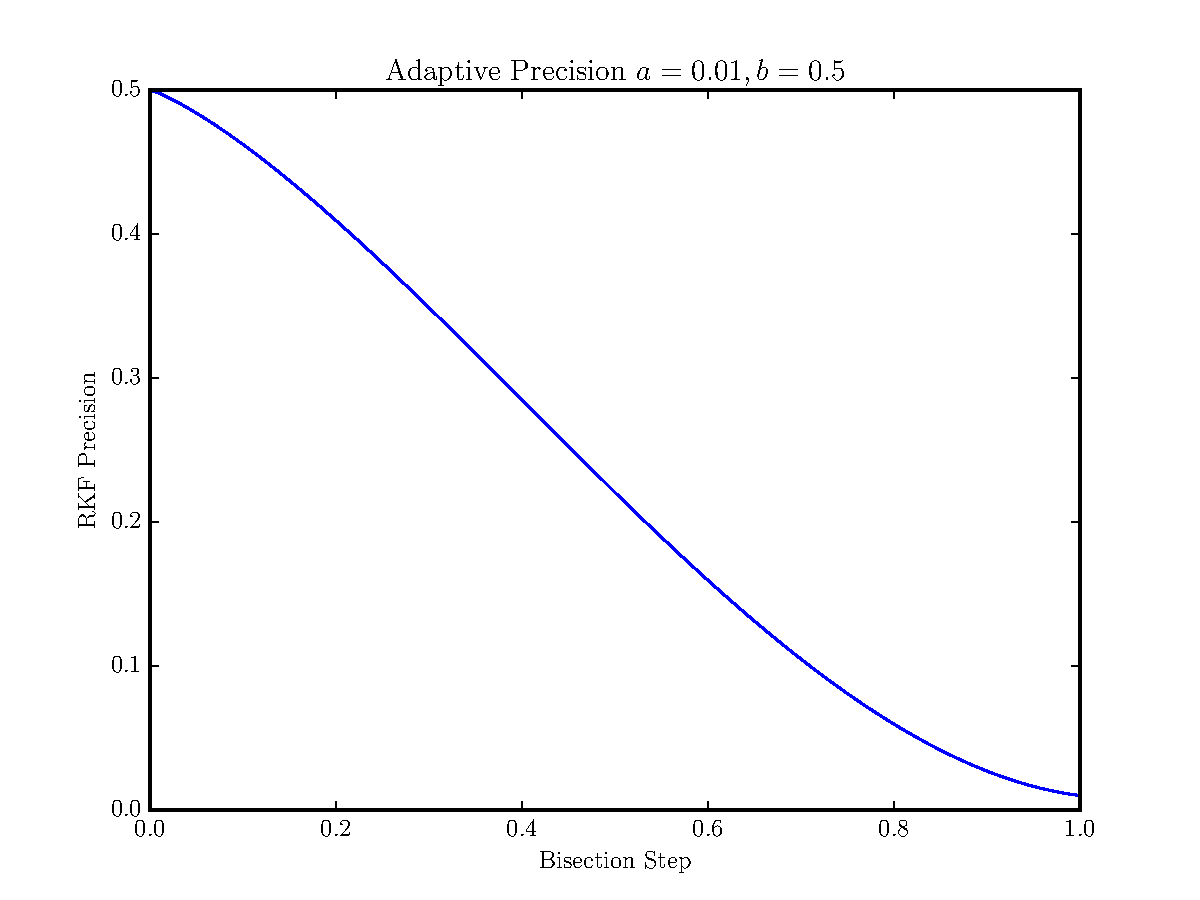
\includegraphics[width=6in]{figures/bisection_tween.pdf}
        \caption{Implementation of adaptive bisection.}
        \label{fig:adaptivebisection}
    \end{figure}
    \end{center}
    \subsubsection{Memory Buffers}
    After successfully computing a new set of stellar state values $\br{\rho,T,M,L}$ for a given radius $r$ using the RKF method, one needs to be careful how to store those values in memory. Below is an example of preallocating chunks of memory in order to store these computed values. $X$ is is a $4\times n$ matrix of stellar state values and $T$ is a $1\times n$ vector for the radius values. Normally, when the step size is fixed and the stopping conditions are less dynamic, one knows the total size of the matrix $X$ before computing anything. Albeit with adaptive step sizes, this is simply not possible. Therefore the amount of memory allocated needs to grow as the RKF procedure finds more and more values. Afterwards, when the stopping condition is reached, the arrays $X,T$ are truncated to a size that corresponds to the number of accurate values computed. This prevents memory pollution and drastically improves performance of the code.
    \begin{lstlisting}
    # Buffer size
    BUFFER = 2**14 # 16384

    # Initialize arrays that will be returned
    T = np.empty( BUFFER )
    X = np.empty( [s, BUFFER] )

    # Initial condition
    T[0] = t
    X[:,0] = x

    i = 0

    while not stop(i,x,t):
        if i + 1 >= len(T):
            # Increasing buffer if needed
            T = np.hstack((T, np.empty(BUFFER)))
            X = np.hstack((X, np.empty([s, BUFFER])))

    (*@\centerline{\raisebox{-1pt}[0pt][0pt]{$\vdots$}}@*)

    # Truncating arrays to final size
    T = T[0:i]
    X = X[:,0:i]

    # Finished RKF
    return ( T, X )
    \end{lstlisting}
    \subsubsection{Multiprocessing}
    After successfully generating stars for a given central temperature $T_c$, our next task was to generate a main sequence with a few hundreds of stars. Each main sequence had a distinct composition and set of $100$ stars logarithmically spanning a range of central temperatures,
    \[ T_c \in \bs{\SI{5e6}{\K},\SI{3.5e7}{\K}} \]
    With each star taking a few seconds to be solved, the runtime of each main-sequence would be large. Therefore the work was split across as many processor cores as we had access to. We managed to get hold of a $12$-core machine to run $7$ main-sequences each with $100$ stars. Python's multiprocessing libraries split up processes by serializing the objects involved. Therefore the star objects generated needed to be serialized and de-serialized in order to be compatible with Python's multiprocessing implementation. The was done using custom-made libraries and not is discussed here. Below is our implementation:
    \begin{lstlisting}
    N_CORES = multiprocessing.cpu_count() - 1
    PROCESSES_PER_CORE = 1

    class MainSequence():

        def __init__(self, min_core_temp, max_core_temp,composition,num_stars):
            self.min_core_temp = min_core_temp
            self.max_core_temp = max_core_temp
            self.num_stars = num_stars
            self.composition = composition
            self.solved = False

        def star_worker(self, temp_c_vals, out_queue):
            for temp_c in temp_c_vals:
                star = Star(temp_c = temp_c, composition=self.composition)
                star.solve()
                star_pickle = {}
                for attribute in star_attributes_to_pickle:
                    star_pickle[attribute] = getattr(star, attribute)
                out_queue.put(star_pickle)
                if LOG: printProgress(out_queue.qsize(), self.num_stars, "Workers")

        @timing
        def solve_stars(self):
            stars = []
            out_queue = Queue()
            num_processes = N_CORES * PROCESSES_PER_CORE
            stars_per_process = np.ceil(self.num_stars / num_processes)
            temp_c_space = np.linspace(start=self.min_core_temp,stop=self.max_core_temp,num=self.num_stars)
            processes = []
            i = 0
            if LOG: printProgress(0, self.num_stars, "Workers")
            while i < self.num_stars:
                remaining_stars = self.num_stars - i
                batch = min(remaining_stars, stars_per_process)
                process = Process(target=self.star_worker, args=(temp_c_space[i:i + batch], out_queue))
                processes.append(process)
                process.start()
                i += batch

            for i in xrange(self.num_stars):
                star = DotDict(out_queue.get())
                stars.append(star)

            for process in processes:
                process.join()

            if LOG: printProgress(self.num_stars, self.num_stars, "Workers")

            self.stars = stars
            self.temp_surf = np.array([star.temp_surf for star in self.stars])
            self.lumin_surf = np.array([star.lumin_surf for star in self.stars])
            self.n_lumin_surf = self.lumin_surf / L_s
            self.mass_surf = np.array([star.mass_surf for star in self.stars])
            self.n_mass_surf = self.mass_surf / M_s
            self.r_surf = np.array([star.r_surf for star in self.stars])
            self.n_r_surf = self.r_surf / R_s
            self.solved = True
    \end{lstlisting}
    \subsubsection{Failures}
    Finally, two other techniques used that offered little to no performance increase under this application where functional caching and pooling of resources. Functional caching is beneficial for functions with no side affects that are called hundreds of times with \textit{same parameters}. For example on each integration step, the energy transport equation \eqref{eq:energytransport} is called a couple of times. Moreover in regions of the star where state values remain virtually constant, functional caching can be used. As an illustration, say there is a function $g\br{x,y,z}$ that takes a few seconds to compute. If the result of $g$ was just computed for $\br{x_1,y_1,z_1}$ and then later in the procedure needs to be computed again with the same parameters, one can re-use the results from before to save time. To do this, each function has an associated hash table with stored parameters and results. This is a rather high-level operation that was seen to have no noticeable impact on the code. Secondly, pooling the star objects provided no benefit to the performance or runtime of the code. These techniques are simply not necessary to achieve efficient running times.
    \section{Results and Analysis}
    Now that the modeling and techniques have been discussed, the results of this project can be reviewed. All convective regions are high-lighted in gray.
    \subsection{Varying Mass}
    \label{sec:varyingmass}
    Before changing metallicity $Z$, we examined two case study stars. One with a mass $M > 2 M_\odot$ and one with a mass less than $M <0.75 M_\odot$. As discussed, the methods used to obtain stellar solutions do not permit one to set the mass of the star explicitly; only the central temperature. Therefore to obtain high-mass stars and low-mass stars, the central temperature $T_c$ was increased and decreased respectively until the desired mass range was obtained. These are the obtained results:
    \begin{center}
        \begin{tabular}{|c|c|c|c|c|c|c|c|}
        \hline
        Star & $T_c (\SI{}{\K})$ & $T_* (\SI{}{\K})$ & $\rho_c (\SI{}{\kg \per \m^3})$ & $R_* (\SI{}{\m})$ & $L_* (\SI{}{\W})$ & $M_* (\SI{}{\kg})$ & $Z$\\
        \hline
        Low-mass & $\SI{8.23e+06}{}$ & $\SI{3.38e+03}{}$ & $\SI{6.82e+04}{}$ & $\SI{5.45e+08}{}$ & $\SI{2.76e+25}{}$ & $\SI{1.29e+30}{}$  & $0.02$ \\
        High-mass & $\SI{3.50e+07}{}$ & $\SI{5.16e+04}{}$ & $\SI{5.14e+02}{}$ & $\SI{7.13e+09}{}$ & $\SI{2.56e+32}{}$ & $\SI{1.68e+32}{}$ & $0.02$ \\
        \hline
        \end{tabular}
    \end{center}
    As can be expected, higher mass stars are hotter, larger and more luminous.
    \begin{center}
        \begin{figure}[H]
            \begin{subfigure}{.5\textwidth}
                \centering
                \caption{Low-mass star.}
                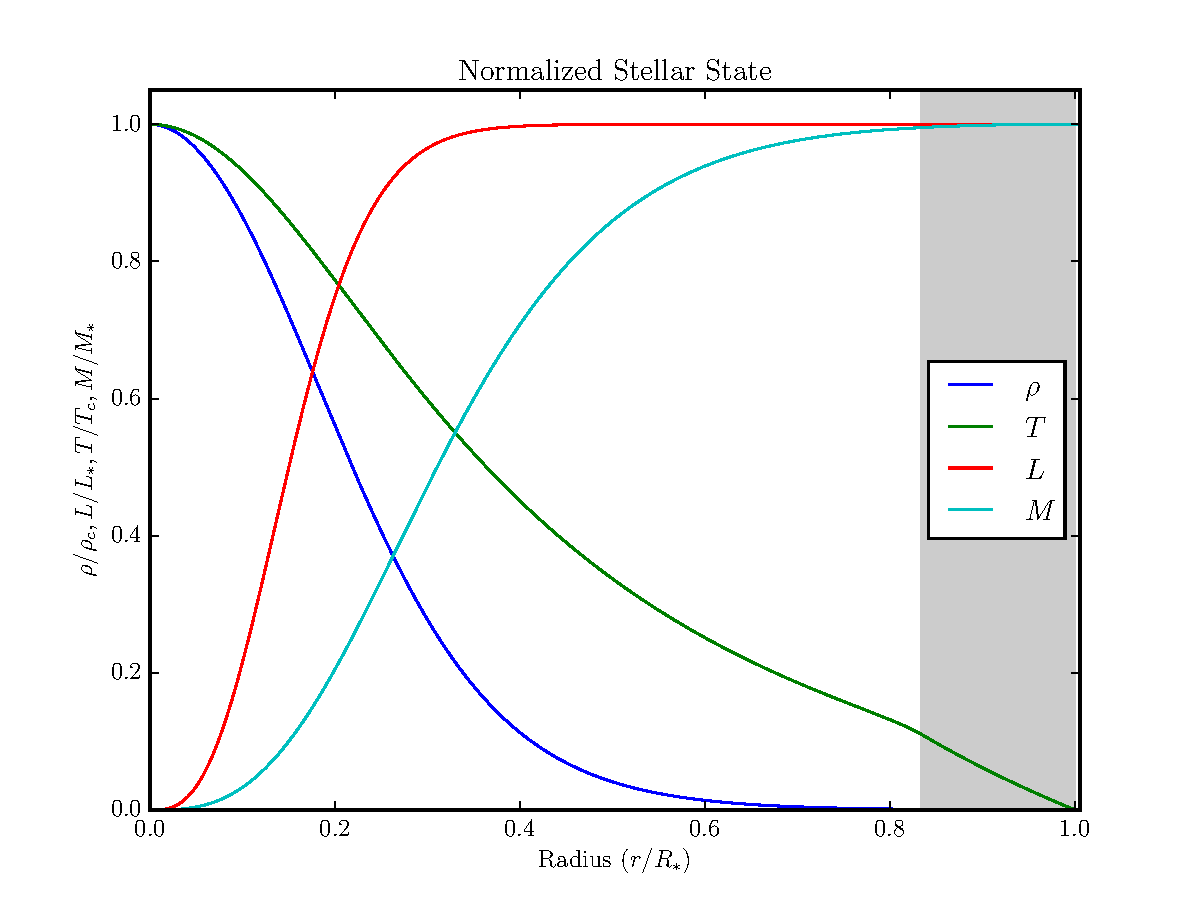
\includegraphics[width=1.1\textwidth]{figures/lowmass/stellar_state.pdf}
                \label{fig:massstarslow}
            \end{subfigure}
            \begin{subfigure}{.5\textwidth}
                \centering
                \caption{High-mass star.}
                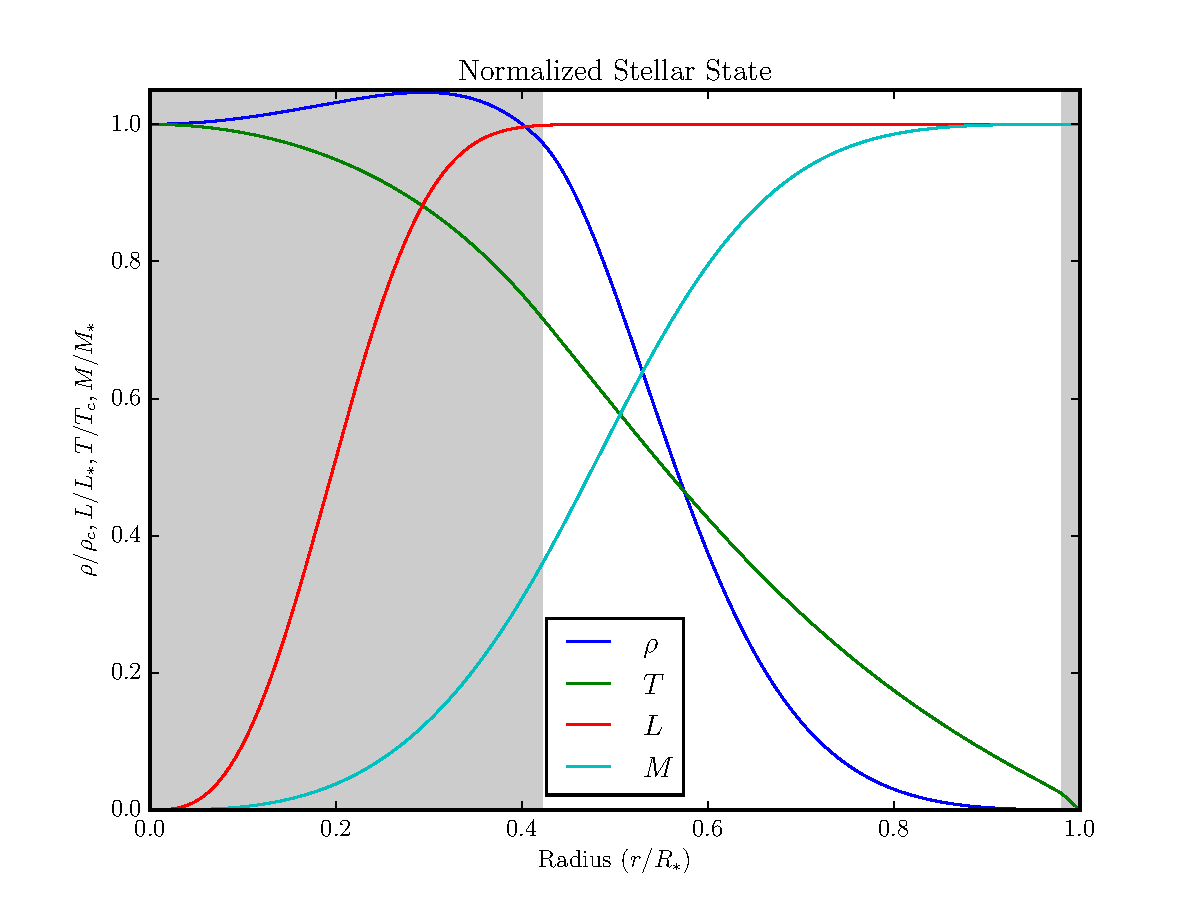
\includegraphics[width=1.1\textwidth]{figures/highmass/stellar_state.pdf}
                \label{fig:massstarshigh}
            \end{subfigure}
            \caption{Comparison of stellar state for different mass stars.}
            \label{fig:stellarstatecomparisonmass}
        \end{figure}
    \end{center}
    When examining figure \ref{fig:stellarstatecomparisonmass}, it is clear that the lower mass star has a radiative core and convective surface. A convective surface is to be expected in all stars will varying degrees since at sufficiently low temperatures at the surface of the star, is becomes harder to transfer energy via radiative transport since it scales with $T^{-3}$ \eqref{eq:energytransport}. In the higher mass star, a large convective core is present. As discussed in section \ref{sec:opacity} this is due to many contributing factors: First, the higher temperatures force radiative pressure to dominate and thus scale with $T^4$ \eqref{eq:partialpressures}. Second, the electron scattering opacity dominates in \eqref{eq:opacitycombo} and finally the CNO cycle dominates energy production at high temperature, increasing luminosity. \\

    Most interestingly, in the convective core of the high mass star, the density increases before falling. This is due to the pressure scaling with $T^4$ due to radiative pressure in \eqref{eq:partialpressures}. As such,
    \[ \abs{\pder{P}{T}\der{T}{r}} > \abs{\f{GM\rho}{r^2}} \implies \der{\rho}{r} > 0 \]
    And the density increases until the temperature decreases enough.
    \begin{center}
        \begin{figure}[H]
            \begin{subfigure}{.5\textwidth}
                \centering
                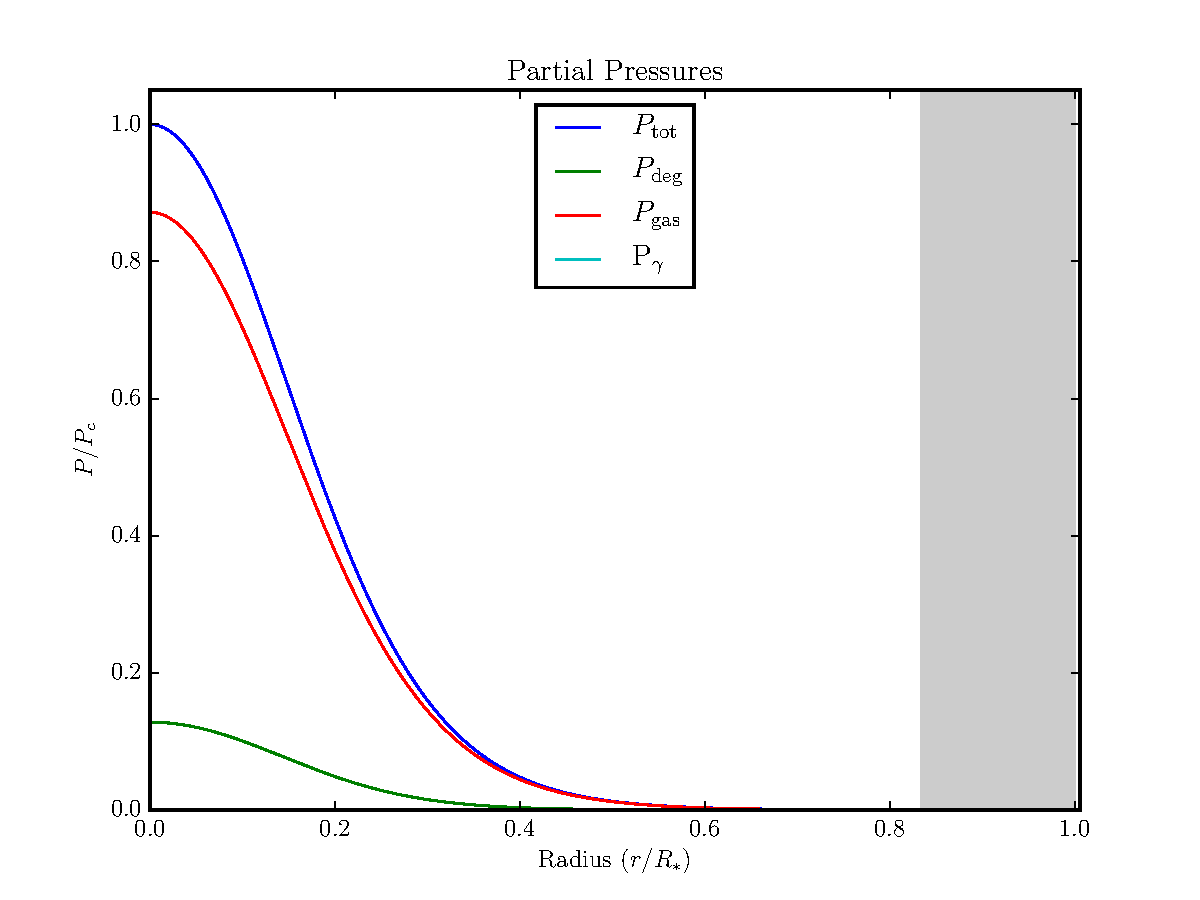
\includegraphics[width=1.1\textwidth]{figures/lowmass/partial_pressure.pdf}
            \end{subfigure}
            \begin{subfigure}{.5\textwidth}
                \centering
                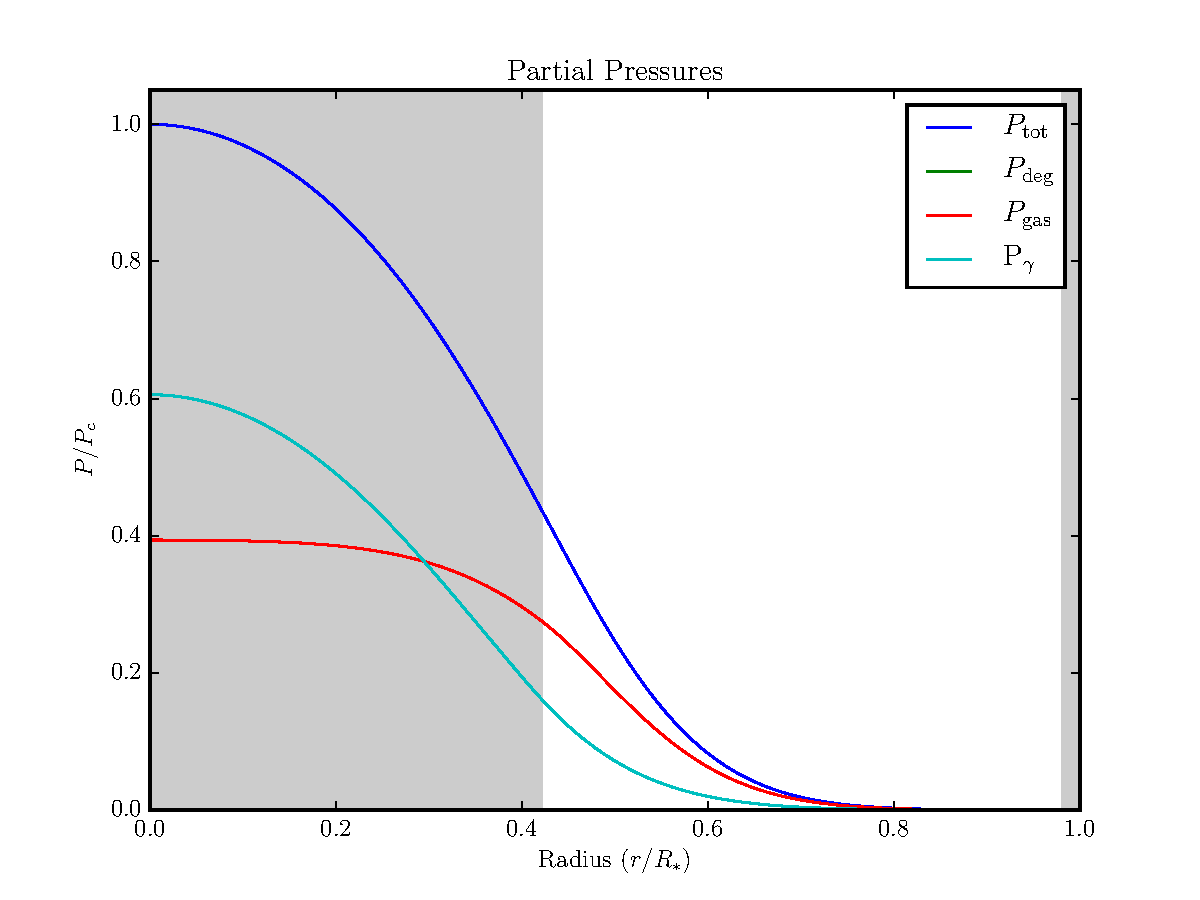
\includegraphics[width=1.1\textwidth]{figures/highmass/partial_pressure.pdf}
            \end{subfigure}
            \caption{Comparison of partial pressures for different mass stars.}
            \label{fig:pressurecomparisonmass}
        \end{figure}
    \end{center}
    As expected, figure \ref{fig:pressurecomparisonmass} illustrates that in the low-mass star, the central temperatures are not high enough for radiative pressure to contribute. In contrast, the high-mass star has a core dominated by photon pressure. Note that degenerate pressure is negligible in the high-mass start due in part to the high temperatures and also to the central density being lower for the high-mass star.
    \begin{center}
        \begin{figure}[H]
            \begin{subfigure}{.5\textwidth}
                \centering
                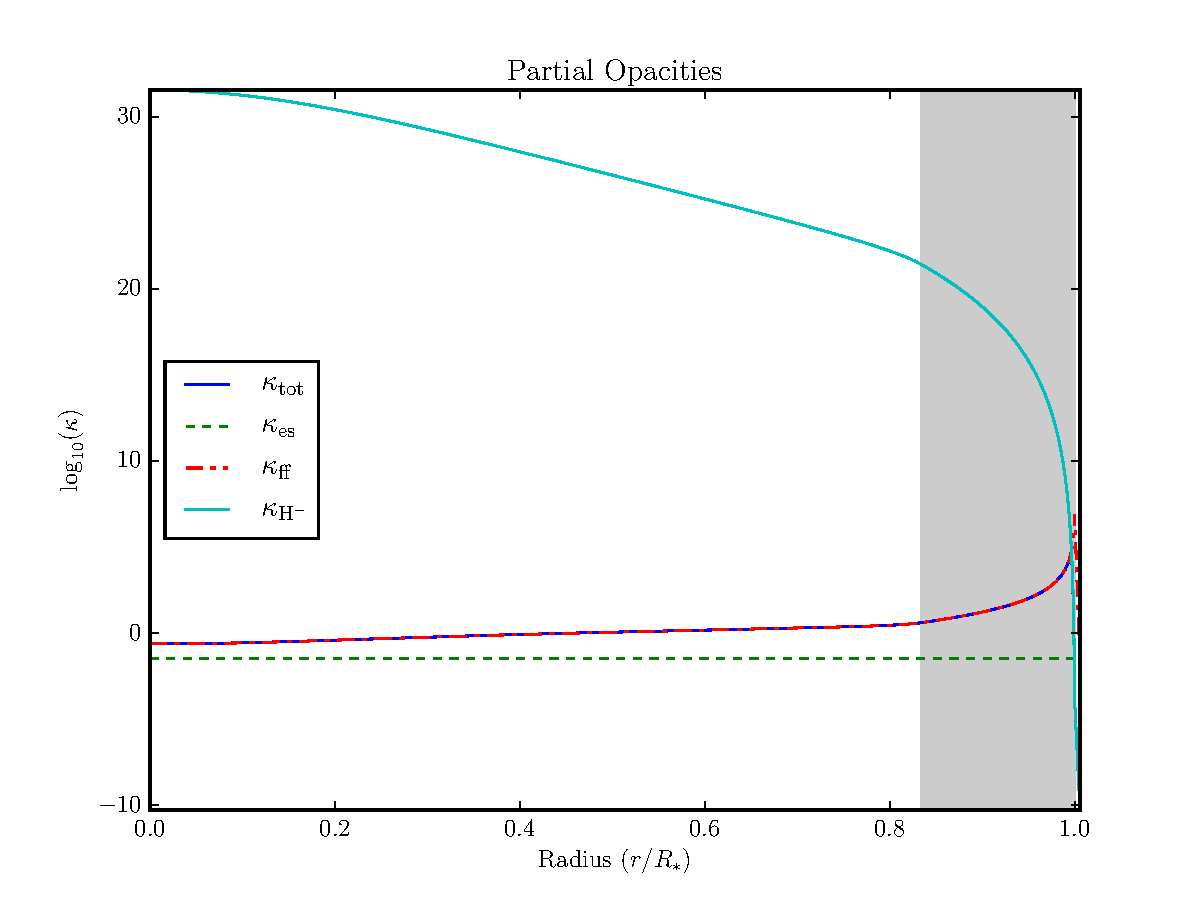
\includegraphics[width=1.1\textwidth]{figures/lowmass/partial_opacity.pdf}
            \end{subfigure}
            \begin{subfigure}{.5\textwidth}
                \centering
                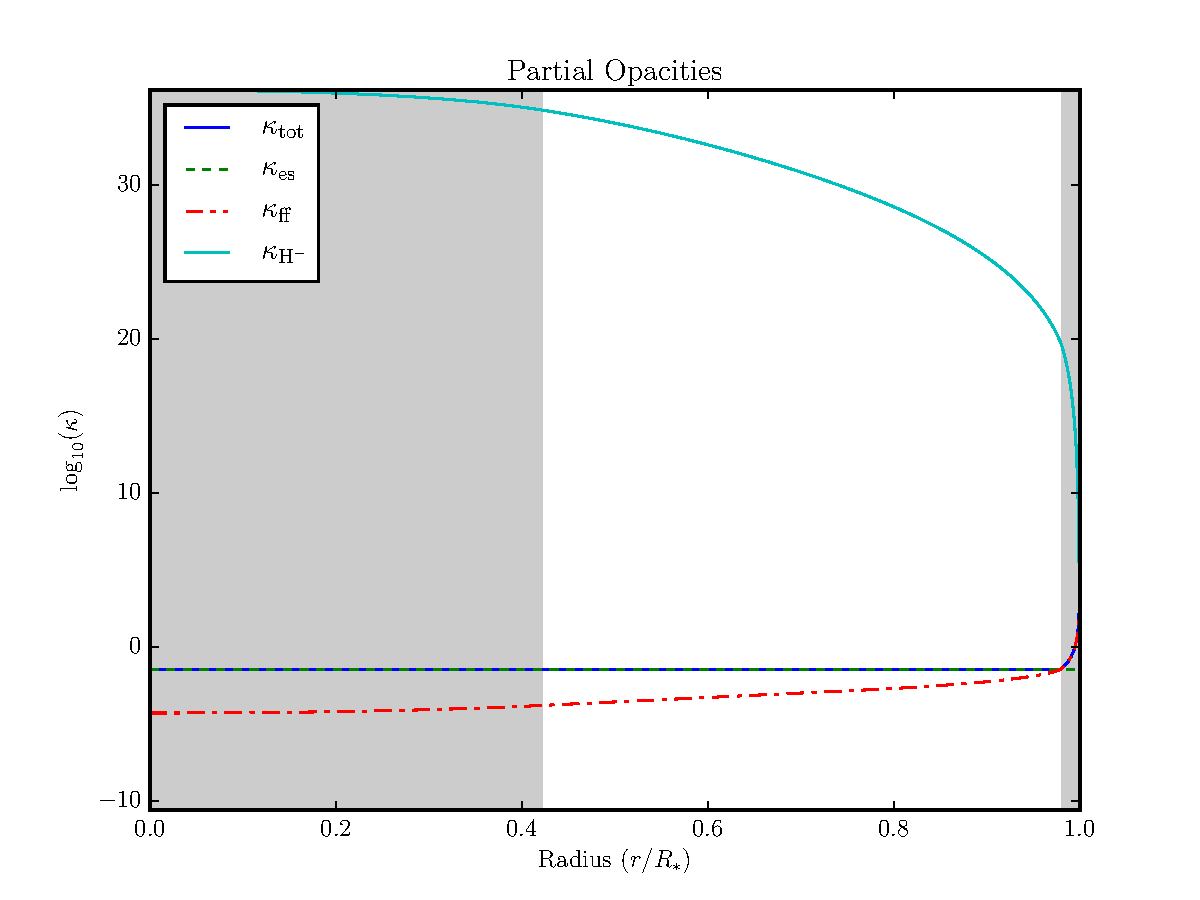
\includegraphics[width=1.1\textwidth]{figures/highmass/partial_opacity.pdf}
            \end{subfigure}
            \caption{Comparison of opacities sources for different mass stars.}
            \label{fig:opacitycomparisonmass}
        \end{figure}
    \end{center}
    Section \ref{sec:opacity} discusses the impact of high temperatures on opacity. In both stars, $\text{H}^-$ opacity only contributes at the surface of the star when neutral hydrogen is present. Figure \ref{fig:opacitycomparisonmass} reveals that at sufficiently high temperatures, electron scattering opacity out-performs free-free opacity. The high-mass star has central opacity purely dominated by electron scattering while the low-mass star has central opacities dominated by electron scattering. We should expect the same effect in low metallicity stars in section \eqref{sec:varyingmetallicity}.
    \begin{center}
        \begin{figure}[H]
            \begin{subfigure}{.5\textwidth}
                \centering
                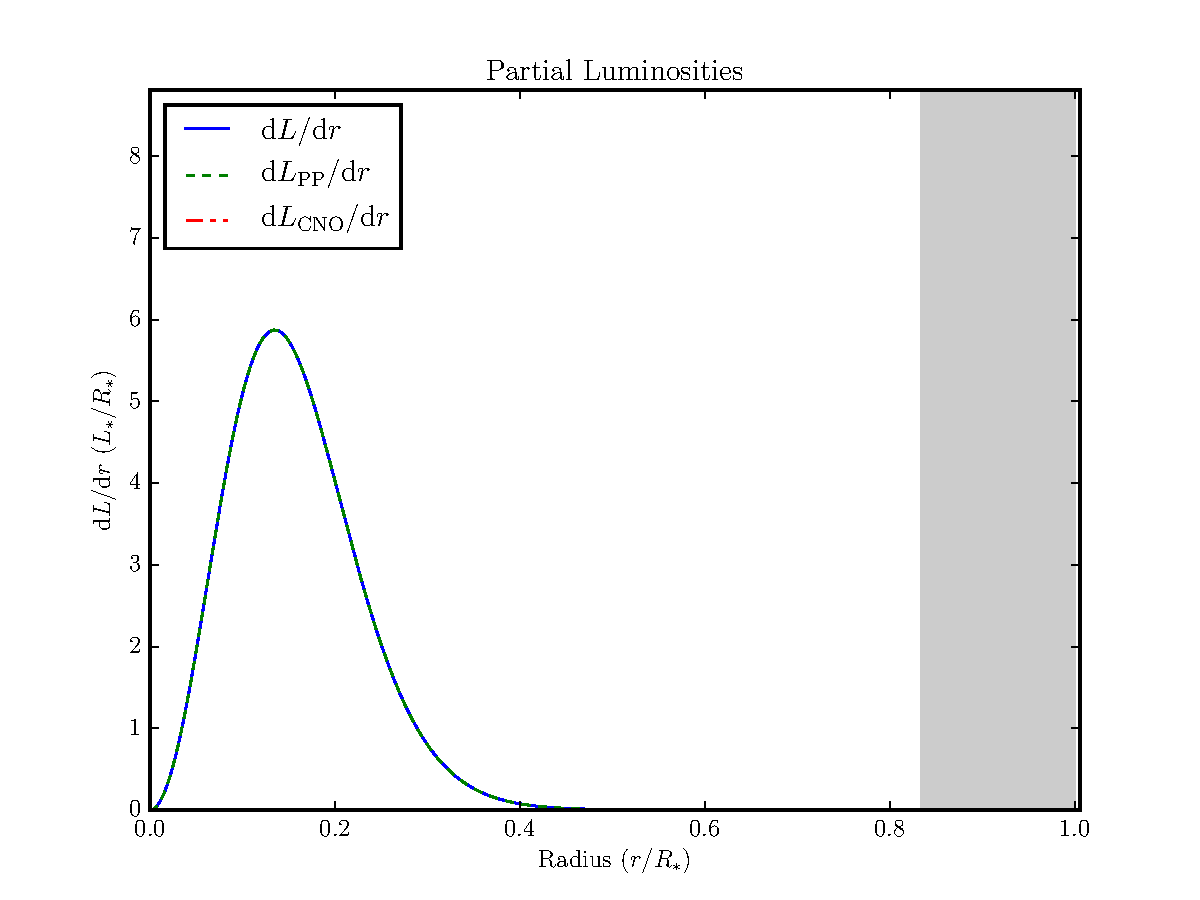
\includegraphics[width=1.1\textwidth]{figures/lowmass/partial_lumin.pdf}
            \end{subfigure}
            \begin{subfigure}{.5\textwidth}
                \centering
                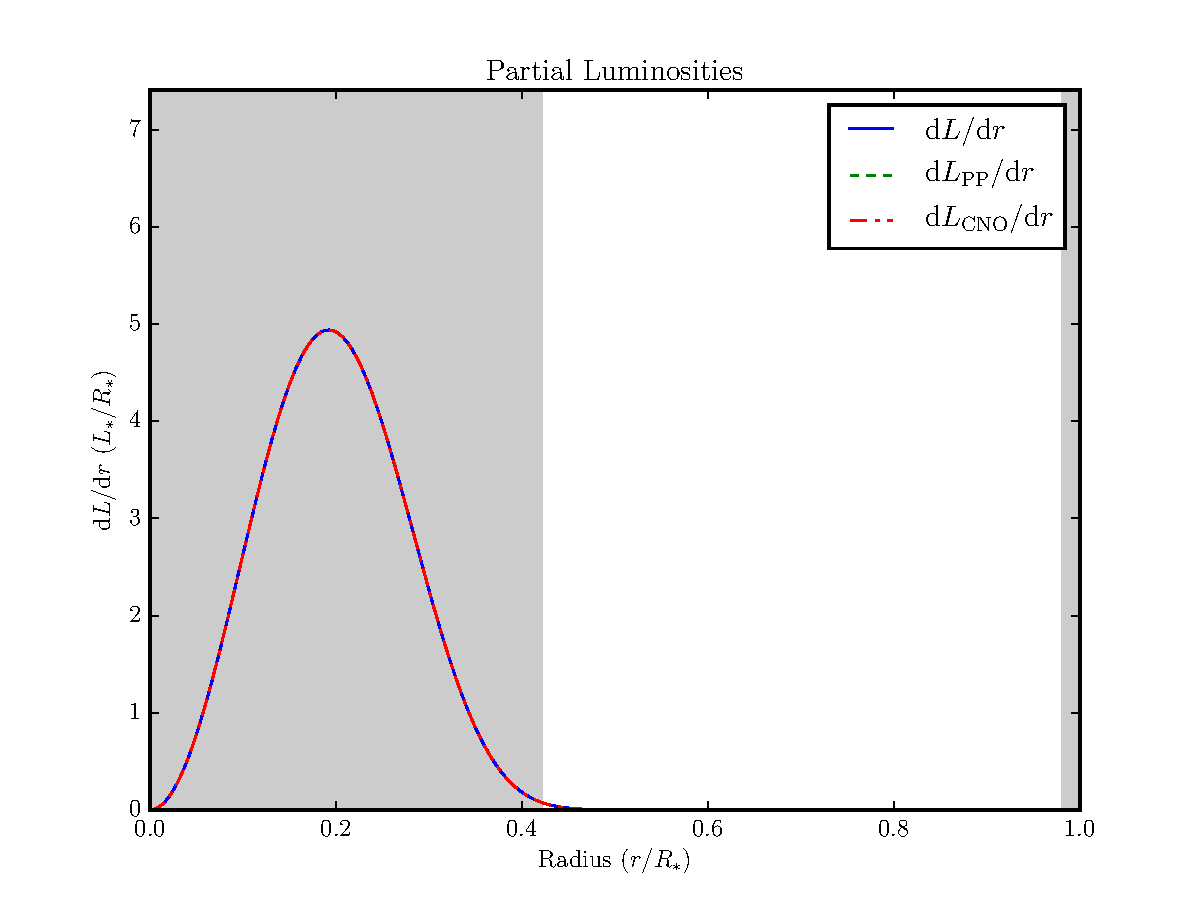
\includegraphics[width=1.1\textwidth]{figures/highmass/partial_lumin.pdf}
            \end{subfigure}
            \caption{Comparison of luminosity sources for different mass stars.}
            \label{fig:luminositycomparisonmass}
        \end{figure}
    \end{center}
    There are two sources of energy production this model is considering: the proton-proton chain and the CNO cycle. Associated energy production rates are given by,
    \[ \ep\tsb{PP} = \SI{1.07e-7}{}\rho_5 X^2 T_6^4 \SI{}{\W\per\kg} \eq \label{eq:ePP}\]
    \[ \ep\tsb{CNO} = \SI{8.24e-26}{}\rho_5 X X\tsb{CNO} T_6^{19.9} \SI{}{\W\per\kg} \eq \label{eq:eCNO}\]
    The important feature being that the proton-proton chain scaling with temperature as $T^4$ \eqref{eq:ePP} and the CNO cycle scaling with temperature as $T^{19.9}$ \eqref{eq:eCNO}. Therefore at higher temperatures, the CNO cycle completely dominates whereas at lower temperatures, the proton-proton chain dominates. Figure \ref{fig:luminositycomparisonmass} is a manifestation of this.

    \begin{center}
        \begin{figure}[H]
            \begin{subfigure}{.5\textwidth}
                \centering
                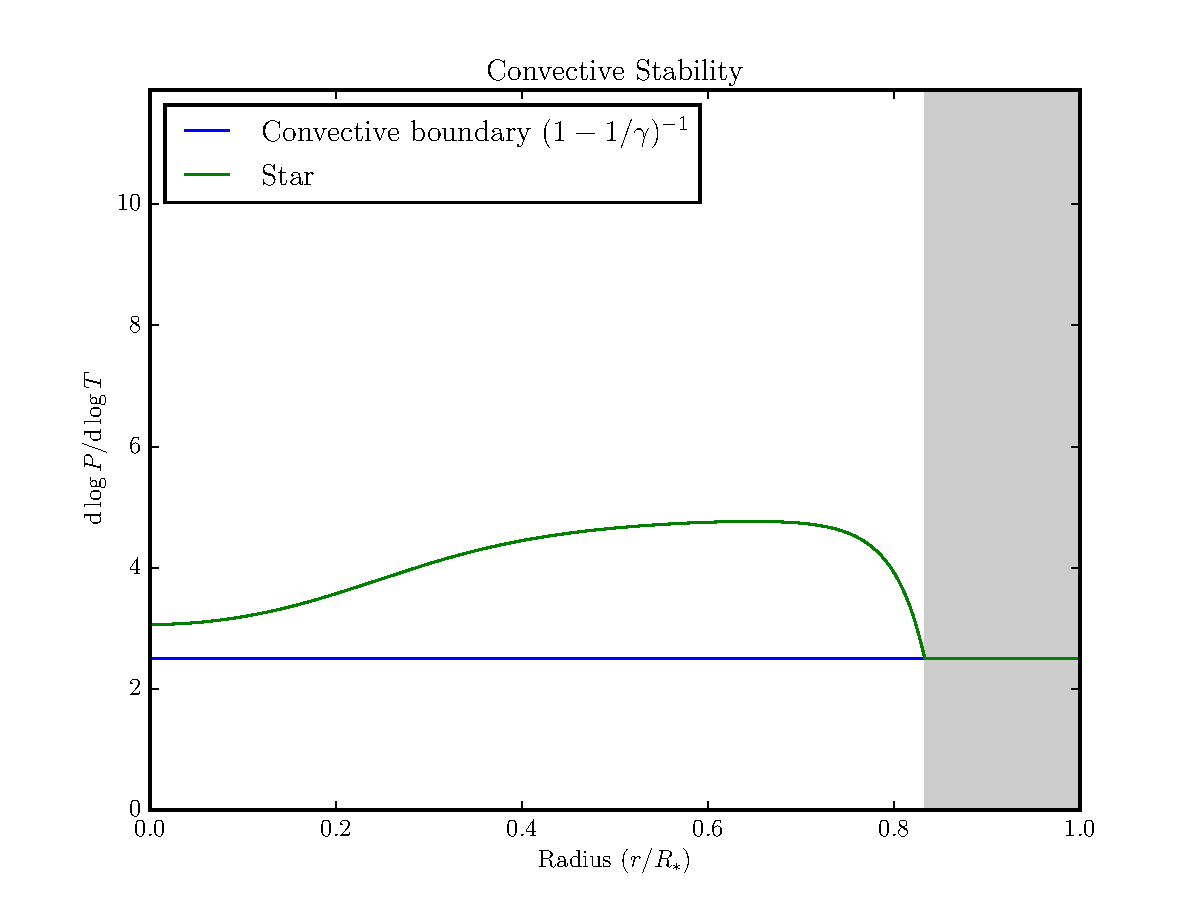
\includegraphics[width=1.1\textwidth]{figures/lowmass/dlogP_dlogT.pdf}
            \end{subfigure}
            \begin{subfigure}{.5\textwidth}
                \centering
                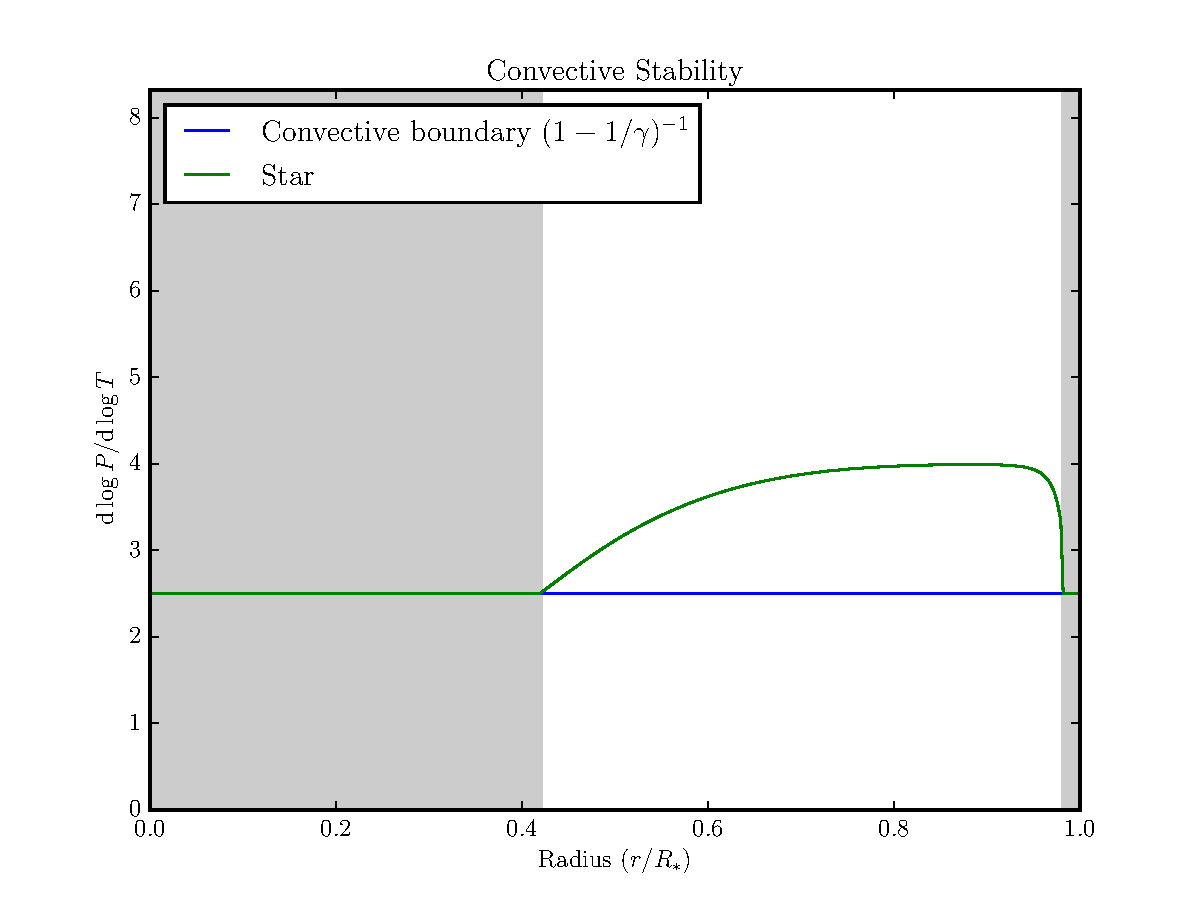
\includegraphics[width=1.1\textwidth]{figures/highmass/dlogP_dlogT.pdf}
            \end{subfigure}
            \caption{Convection zones in different mass stars.}
            \label{fig:convectivecomparisonmass}
        \end{figure}
    \end{center}

    Figure \ref{fig:convectivecomparisonmass} is simply a graph of the convective and radiative zones in the star. When the star is being convective, $\dif \log P / \dif \log T$ is constant. For convection,
    \[ \der{\log P}{\log T} = \f{T}{P}\der{P}{T} = \f{T}{P}\der{P}{r}\der{r}{T} = \f{T}{P}\br{-\f{GM\rho}{r^2}}\br{-\br{1-\f{1}{\ga}}\f{T}{P}\f{GM\rho}{r^2}}^{-1} = \br{1 - \f{1}{\gamma}}^{-1} \]

    \subsection{Varying Metallicity}
    \label{sec:varyingmetallicity}
    Given that the stellar model produced exhibits general stellar properties that are physically motivated, is sufficient to explore more the exotic behavior of high and low metallicity stars. One star was generated with a very small metallicity of $Z = \SI{1e-8}{}$ and one with ten times the solar metallicity $Z = 0.2$. As a note of comparison, each of these stars were generated with the same central temperature of $T_c = \SI{8.23e+06}{\K}$; the same central temperature used for low-mass star in section \ref{sec:varyingmass}. Consequently, the low-mass star with metallicity $Z = 0.02$ can be used as an intermediate metallicity case study if necessary.
    \begin{center}
        \begin{tabular}{|c|c|c|c|c|c|c|c|}
        \hline
        Star & $T_c (\SI{}{\K})$ & $T_* (\SI{}{\K})$ & $\rho_c (\SI{}{\kg \per \m^3})$ & $R_* (\SI{}{\m})$ & $L_* (\SI{}{\W})$ & $M_* (\SI{}{\kg})$ & $Z$\\
        \hline
        Low-Z & $\SI{8.23e+06}{}$ & $\SI{6.49e+03}{}$ & $\SI{2.25e+05}{}$ & $\SI{2.00e+08}{}$ & $\SI{5.06e+25}{}$ & $\SI{7.16e+29}{}$ & $\SI{1e-8}{}$ \\
        High-Z & $\SI{8.23e+06}{}$ & $\SI{2.42e+03}{}$ & $\SI{3.01e+04}{}$ & $\SI{8.16e+08}{}$ & $\SI{1.62e+25}{}$ & $\SI{1.76e+30}{}$ & $0.2$ \\
        \hline
        \end{tabular}
    \end{center}
    The first noticeable feature is that lower metallicity stars are smaller, have higher densities, are hotter and yet more luminous despite the smaller size. The smaller size is a result of the lower opacity \eqref{eq:opacitycombo}. With smaller opacity the optical depth falls faster that normal, meaning the surface of the star is reached much sooner during integration. The optical depth boundary condition \eqref{eq:tauboundary} and associated proxy \eqref{eq:tauproxy} gives the proportionality,
    \[ R_* \propto \kappa \]
    Thus lower metallicity implies lower opacity which in turn yields smaller stars. The higher central density and surface temperature in low metallicity stars is a combination of flatter density and temperature gradients as illustrated in figure \ref{fig:stellarstatecomparisonZ} in conjunction with smaller radius (the temperature and density does not change as much). A higher surface temperature increases surface luminosity; although a smaller size decreased luminosity. Evidently, for low metallicity stars, the luminosity overall increases. Overall, when decreasing the metallicity in a star, one should expect it to move left and upward on a Hertzsprung–Russell as will be seen in section \eqref{sec:mainseq}.
    \begin{center}
        \begin{figure}[H]
            \begin{subfigure}{.5\textwidth}
                \centering
                \caption{Low-Z star.}
                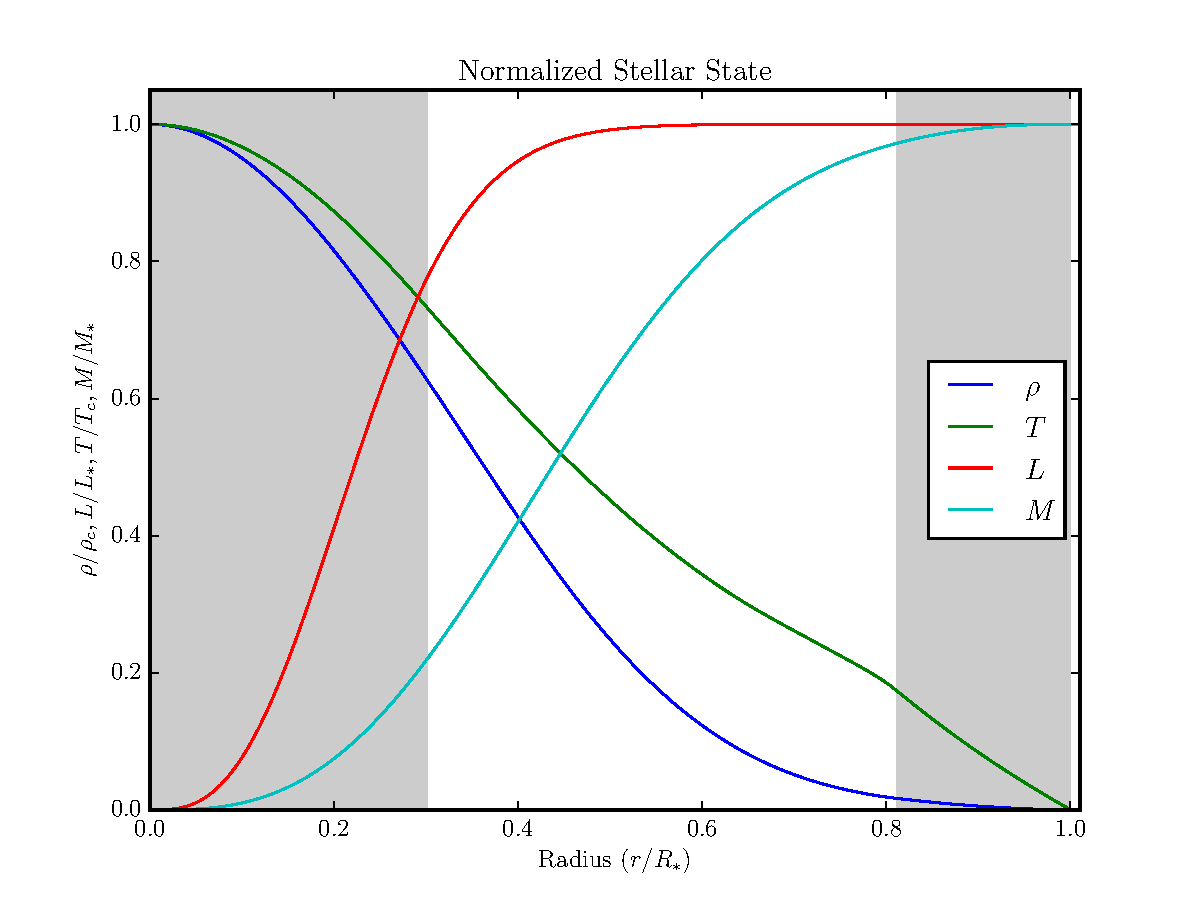
\includegraphics[width=1.1\textwidth]{figures/lowZ/stellar_state.pdf}
                \label{fig:Zstarslow}
            \end{subfigure}
            \begin{subfigure}{.5\textwidth}
                \centering
                \caption{High-Z star.}
                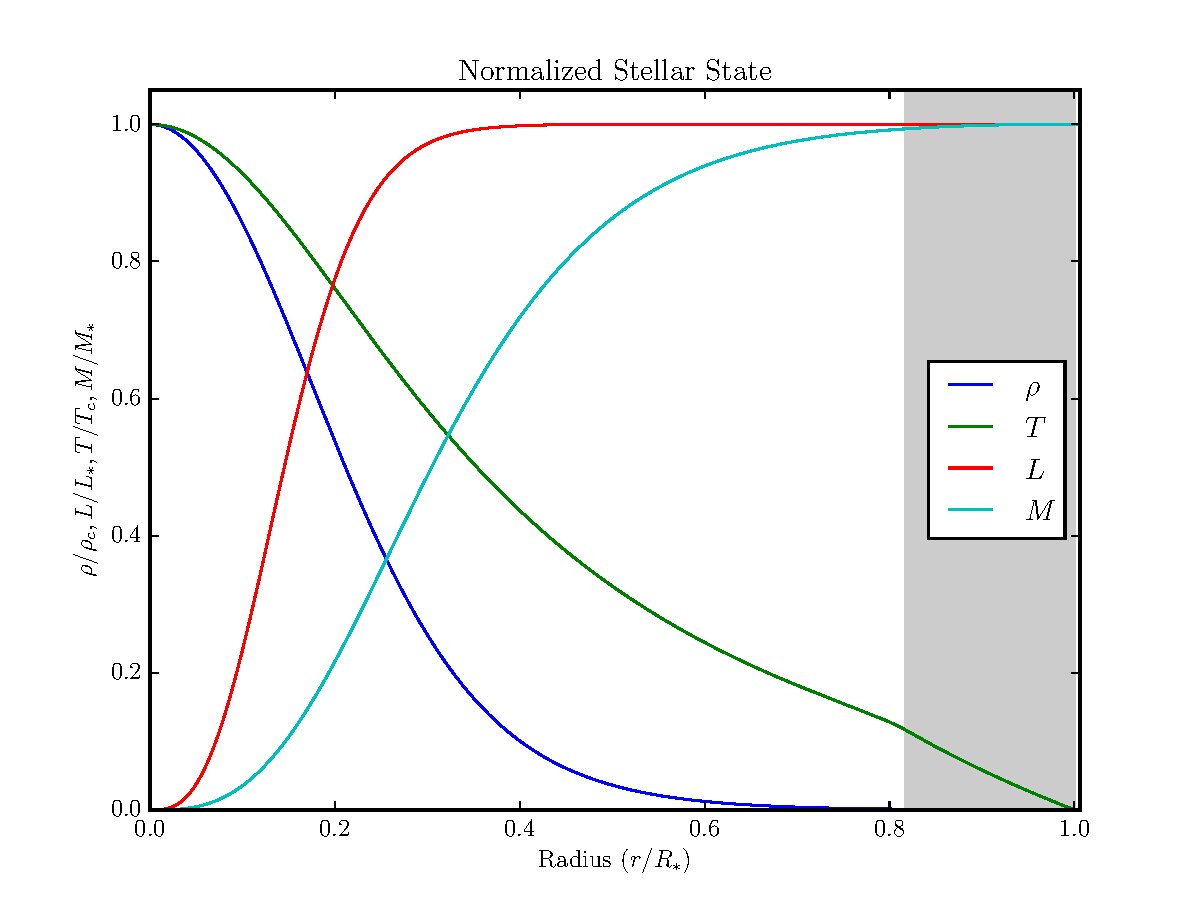
\includegraphics[width=1.1\textwidth]{figures/highZ/stellar_state.pdf}
                \label{fig:Zstarshigh}
            \end{subfigure}
            \caption{Comparison of stellar state for different Z stars.}
            \label{fig:stellarstatecomparisonZ}
        \end{figure}
    \end{center}
    The convective core in the lower metallicity star is a result of electron scattering opacity dominating in the center of the star as discussed in section \ref{sec:opacity}. In contrast to higher temperature stars, lower metallicity stars develop convective cores while increasing the central density instead of decreasing central density as in high temperature stars.
    \begin{center}
        \begin{figure}[H]
            \begin{subfigure}{.5\textwidth}
                \centering
                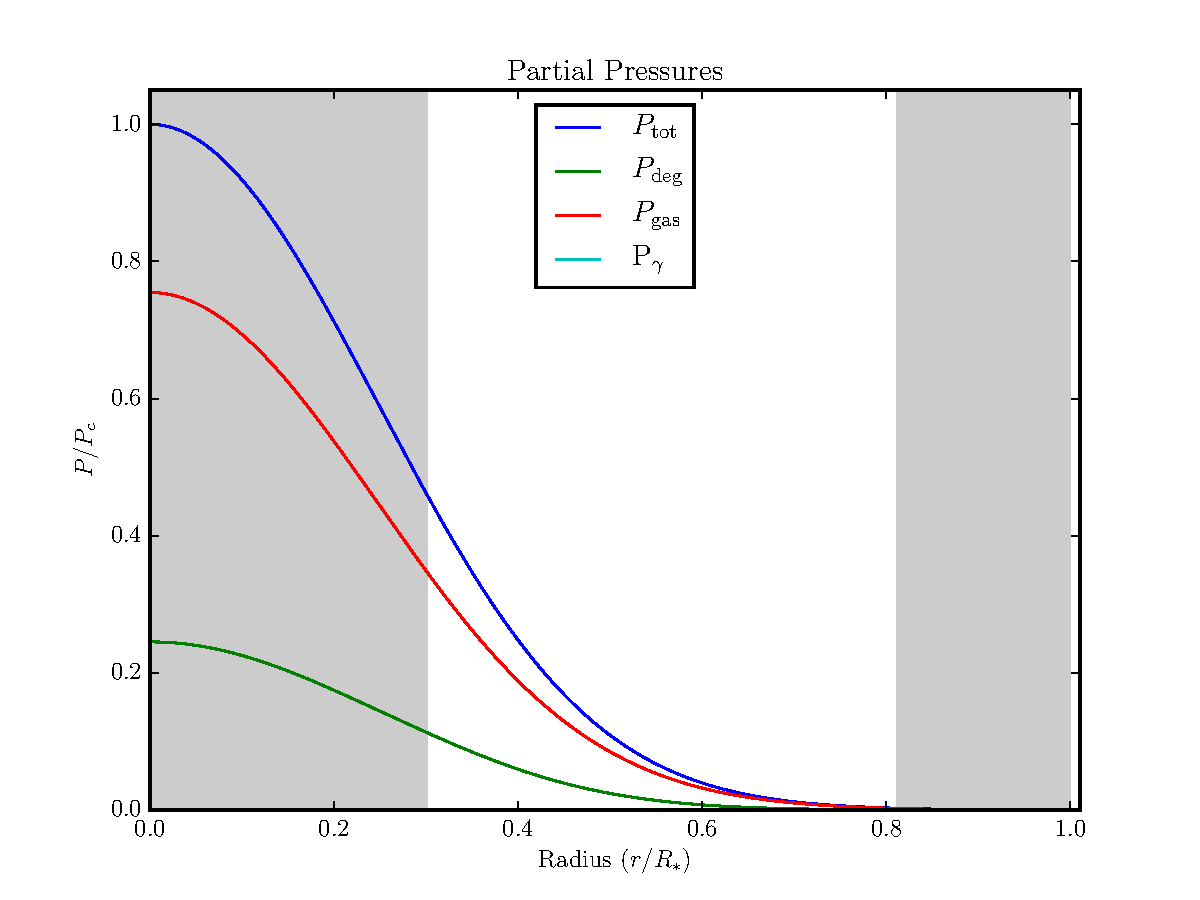
\includegraphics[width=1.1\textwidth]{figures/lowZ/partial_pressure.pdf}
            \end{subfigure}
            \begin{subfigure}{.5\textwidth}
                \centering
                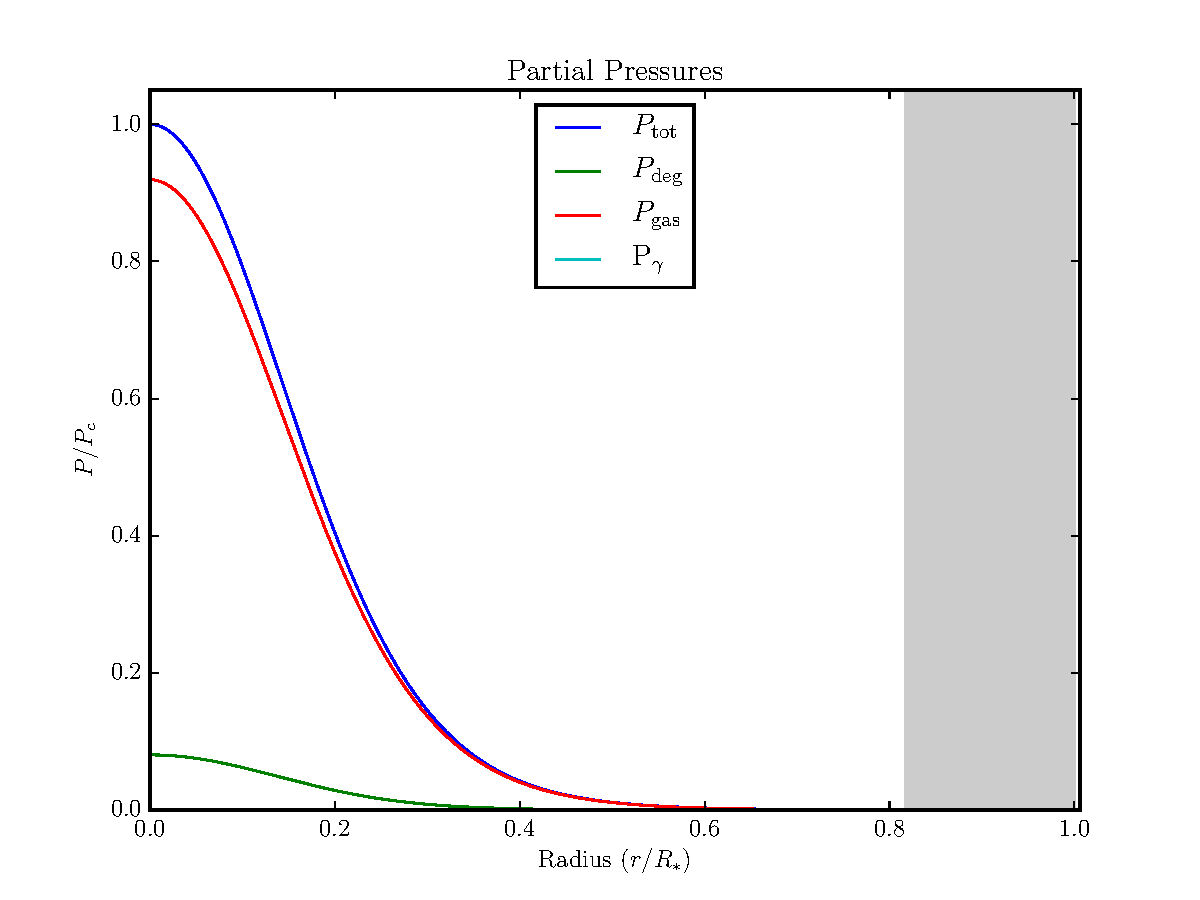
\includegraphics[width=1.1\textwidth]{figures/highZ/partial_pressure.pdf}
            \end{subfigure}
            \caption{Comparison of partial pressures for different Z stars.}
            \label{fig:pressurecomparisonZ}
        \end{figure}
    \end{center}
    As expected, figure \ref{fig:pressurecomparisonZ} shows that ideal gas pressure is dominant in both the high metallicity and low metallicity star due to the moderate to small central temperature. Notice that in the low metallicity star with higher central density, the degeneracy pressure begins to contribute a more as the particles are packed closer and closer in phase space.
    \begin{center}
        \begin{figure}[H]
            \begin{subfigure}{.5\textwidth}
                \centering
                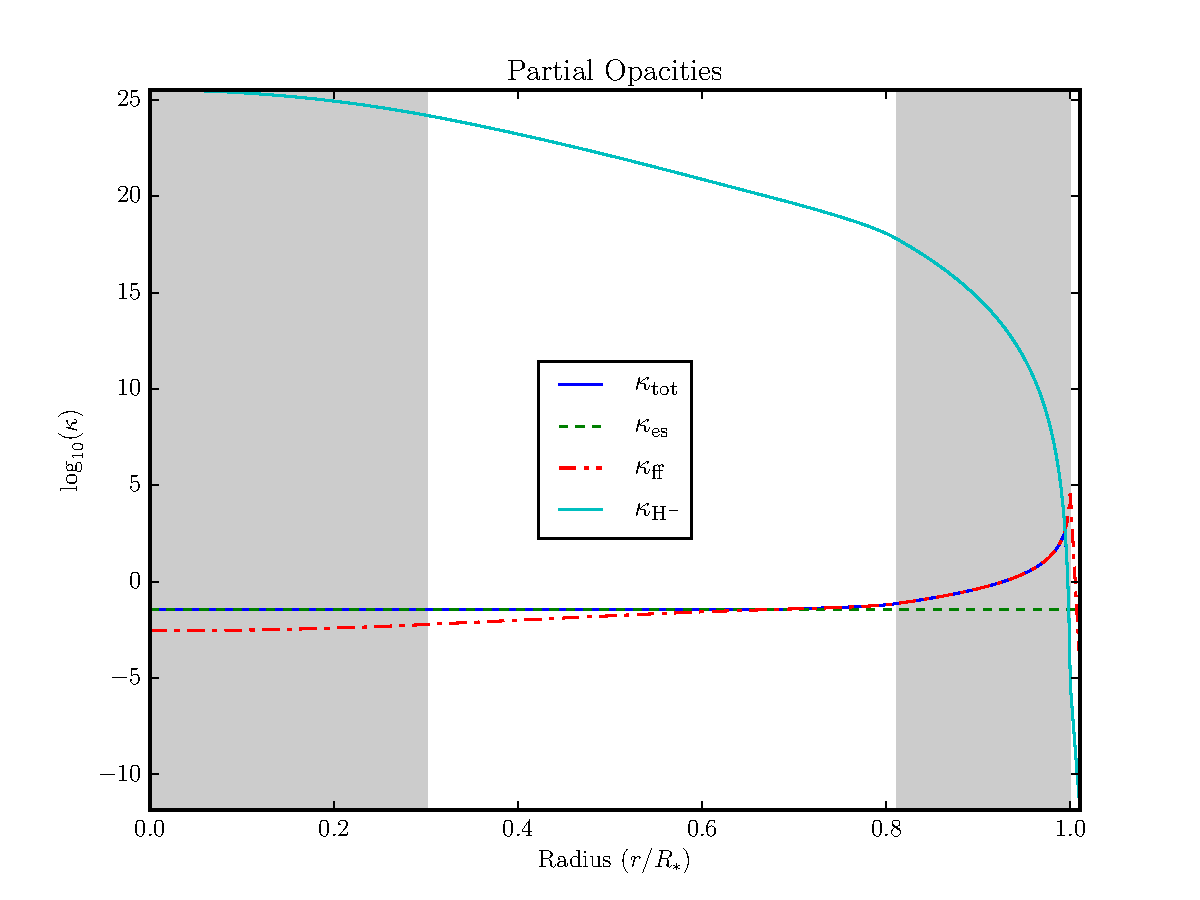
\includegraphics[width=1.1\textwidth]{figures/lowZ/partial_opacity.pdf}
            \end{subfigure}
            \begin{subfigure}{.5\textwidth}
                \centering
                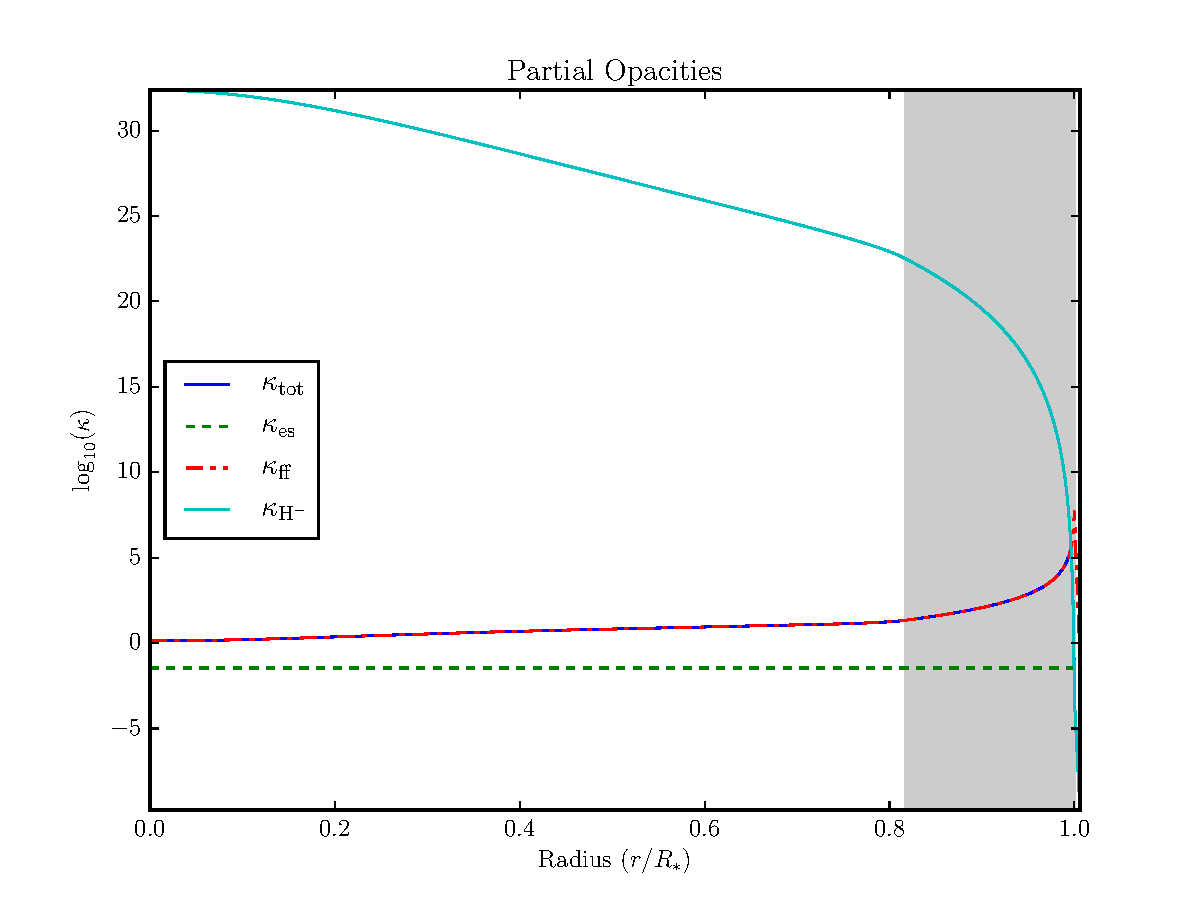
\includegraphics[width=1.1\textwidth]{figures/highZ/partial_opacity.pdf}
            \end{subfigure}
            \caption{Comparison of opacities sources for different Z stars.}
            \label{fig:opacitycomparisonZ}
        \end{figure}
    \end{center}
    Figure \ref{fig:opacitycomparisonZ} illustrates exactly the phenomena discussed in section \ref{sec:opacity}. At sufficiently low metallicity, the free-free opacity sources decrease in strength until electron scattering components dominate, holding the opacity constant in the center of the star.
    \begin{center}
        \begin{figure}[H]
            \begin{subfigure}{.5\textwidth}
                \centering
                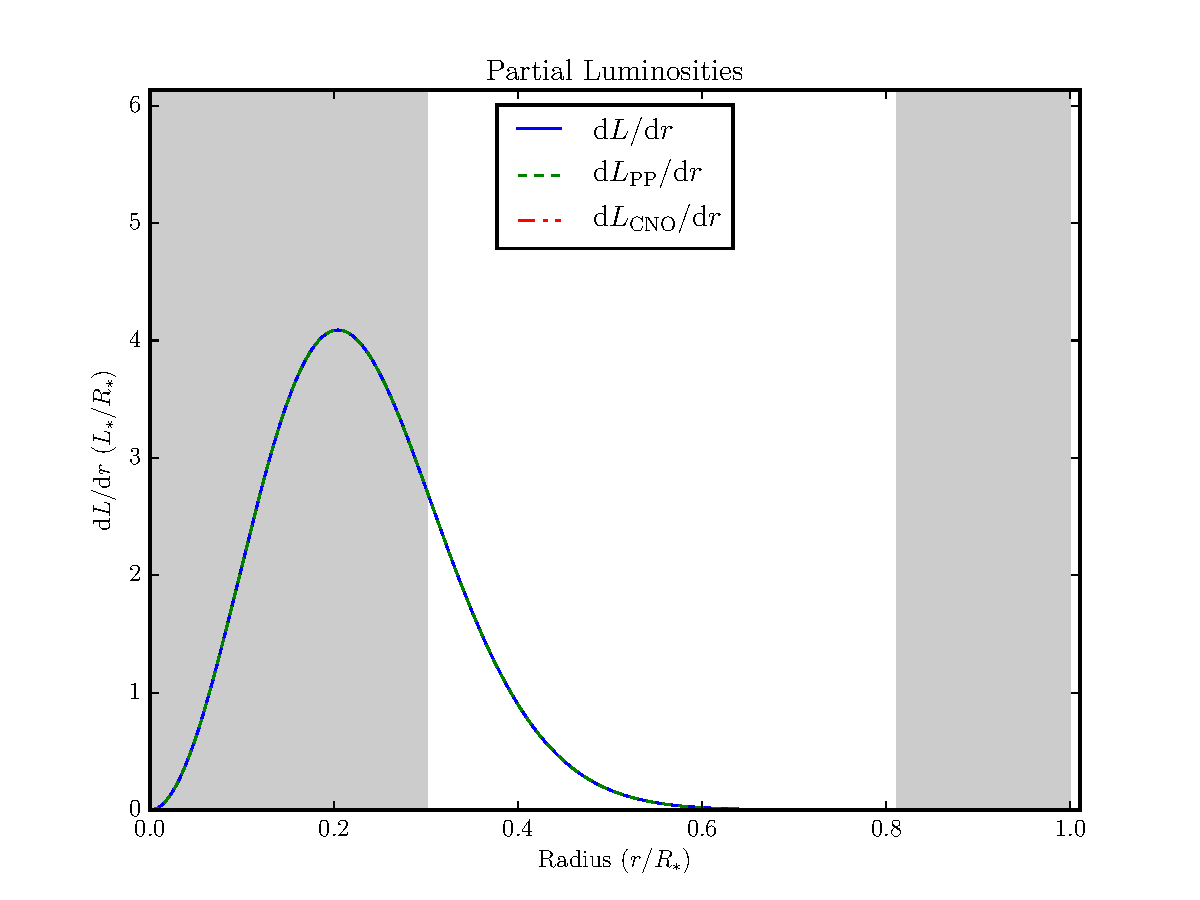
\includegraphics[width=1.1\textwidth]{figures/lowZ/partial_lumin.pdf}
            \end{subfigure}
            \begin{subfigure}{.5\textwidth}
                \centering
                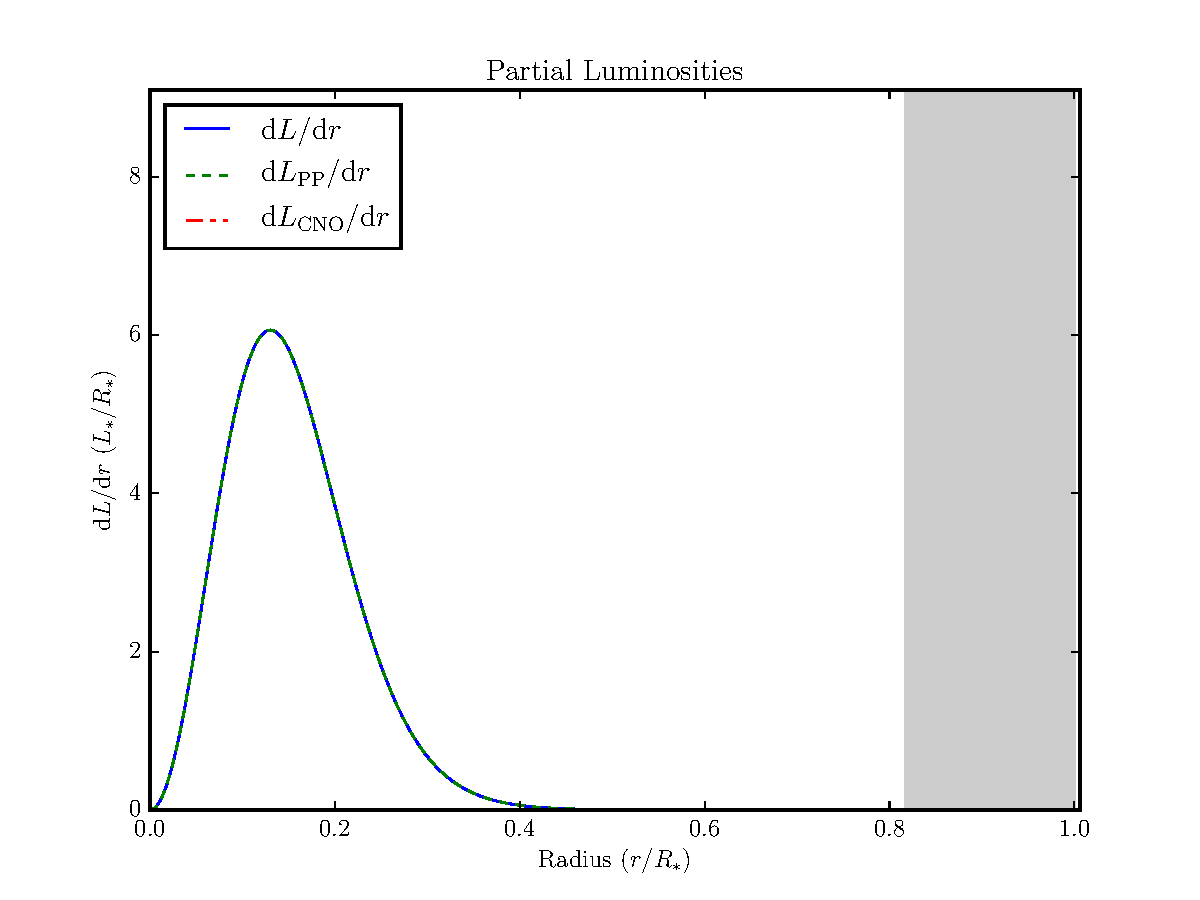
\includegraphics[width=1.1\textwidth]{figures/highZ/partial_lumin.pdf}
            \end{subfigure}
            \caption{Comparison of luminosity sources for different Z stars.}
            \label{fig:luminositycomparisonZ}
        \end{figure}
    \end{center}
    Since both stars have central temperatures that are comparatively low, only the proton-proton chain contributes to energy production as seen in figure \ref{fig:luminositycomparisonZ}. At higher temperatures, the CNO cycle would contribute more. This effective is entirely independent of the metallicity $Z$ for fixed $X$.
    \begin{center}
        \begin{figure}[H]
            \begin{subfigure}{.5\textwidth}
                \centering
                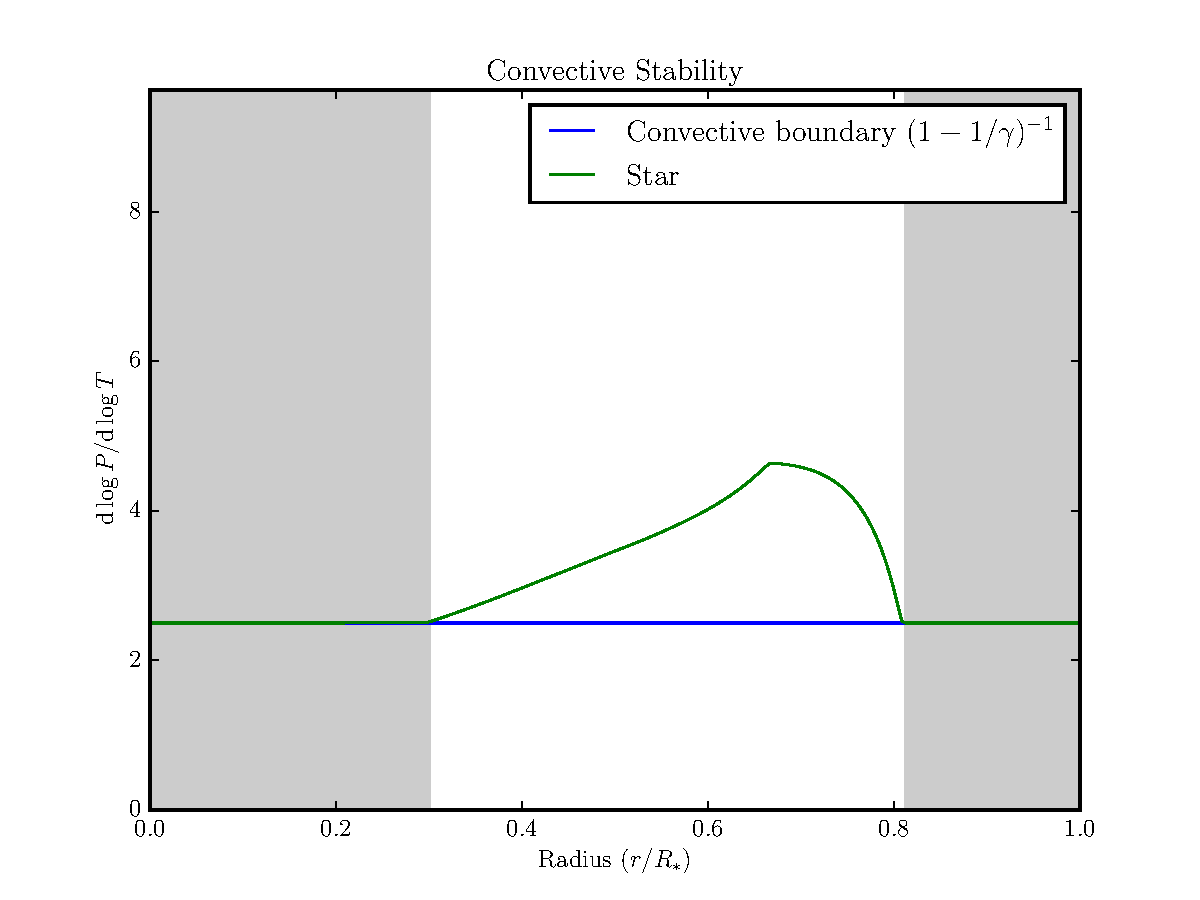
\includegraphics[width=1.1\textwidth]{figures/lowZ/dlogP_dlogT.pdf}
            \end{subfigure}
            \begin{subfigure}{.5\textwidth}
                \centering
                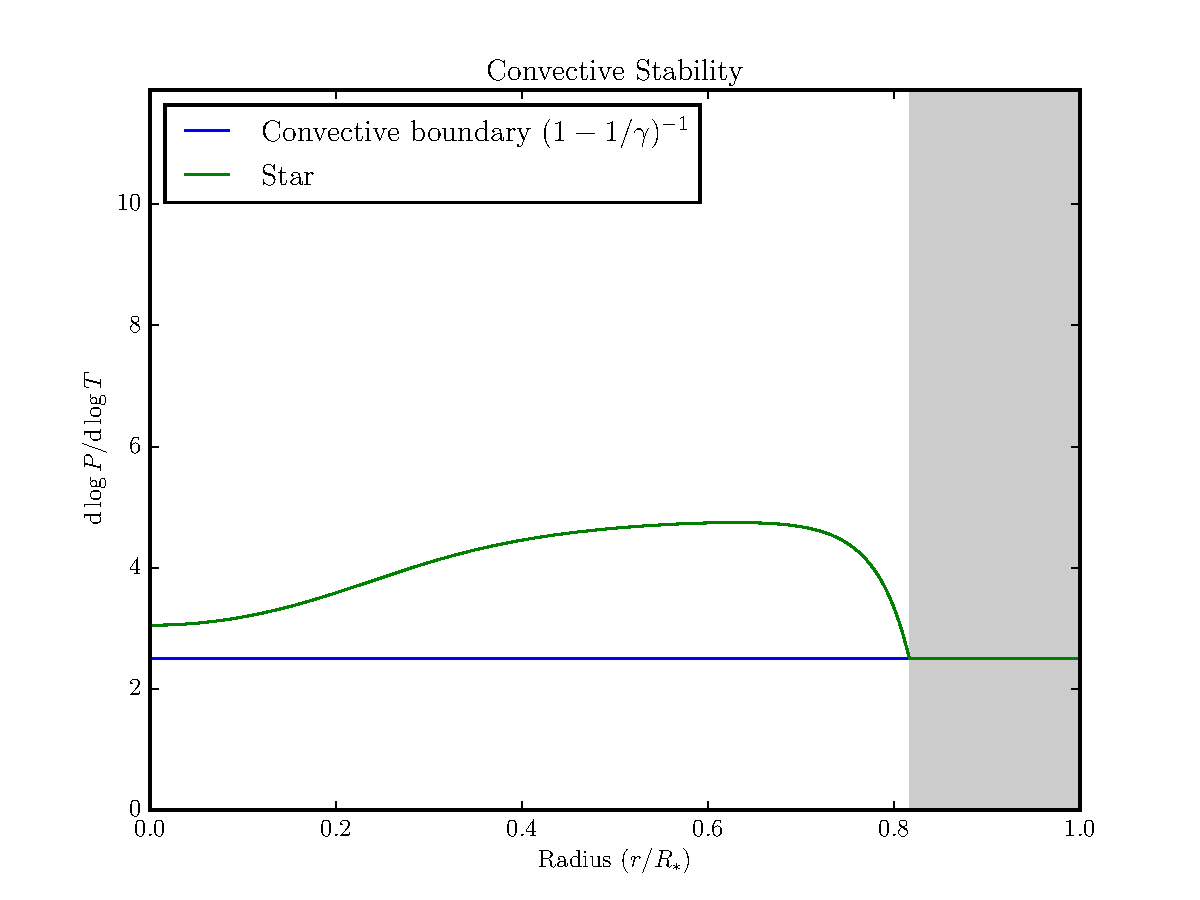
\includegraphics[width=1.1\textwidth]{figures/highZ/dlogP_dlogT.pdf}
            \end{subfigure}
            \caption{Convection zones in different Z stars.}
            \label{fig:convectivecomparisonZ}
        \end{figure}
    \end{center}
    \subsection{Main Sequence}
    \label{sec:mainseq}
    Figure \ref{fig:ms} is a plot of $7$ main sequences with varying metallicity. As a reminder, each is taken to have $X = X_\odot = 0.73$. As anticipated from the analysis of \eqref{sec:varyingmetallicity}, lower metallicity stars are more luminosity and hotter (bluer). Figure \ref{fig:RvM} reveals that lower metallicity, population III stars are smaller than population II and I stars. Figure \ref{fig:LvM} demonstrates how population III stars are more luminous than stars of the same mass. Moreover, population II and I stars ($Z \geq 0.0001$) live roughly in the domain of empirical measurement. This is not unexpected; we have observed both population II and I stars. In some cases, if it were not for spectroscopic measurements, solar metallicity stars $Z = 0.02$ would be indistinguishable from higher metallicity stars $Z = 0.2$ as they share nearly identical parameterizations (particularly at higher temperatures where their branches converge on one another). \\

    Figure \ref{fig:ms} illuminates numerous reasons why population III stars are difficult to observe if they were to exist. Older, population III stars are more luminous. This combination indicates that population III stars would have likely died out a long time ago. As such, we would have to look extremely far into space and into the past to observe these bright blue stars while they still existed. It gets worse; when looking at very distant stars, astronomers have a bias for the brighter, higher temperature stars. Figure \ref{fig:ms}, specifically the $Z = 1e-11$ branch ``rejoins'' the main sequences at higher temperatures. These stars would be indistinguishable from normal, main-sequence stars on a Hertzsprung–Russell diagram. The best candidates for the first observed population III stars will be very luminous and have very, very low metallicities ($Z<1e-16$) when they become distinguishable from the main-sequence and have branch-slopes smaller than the main-sequence.
    \begin{center}
        \begin{figure}[H]
            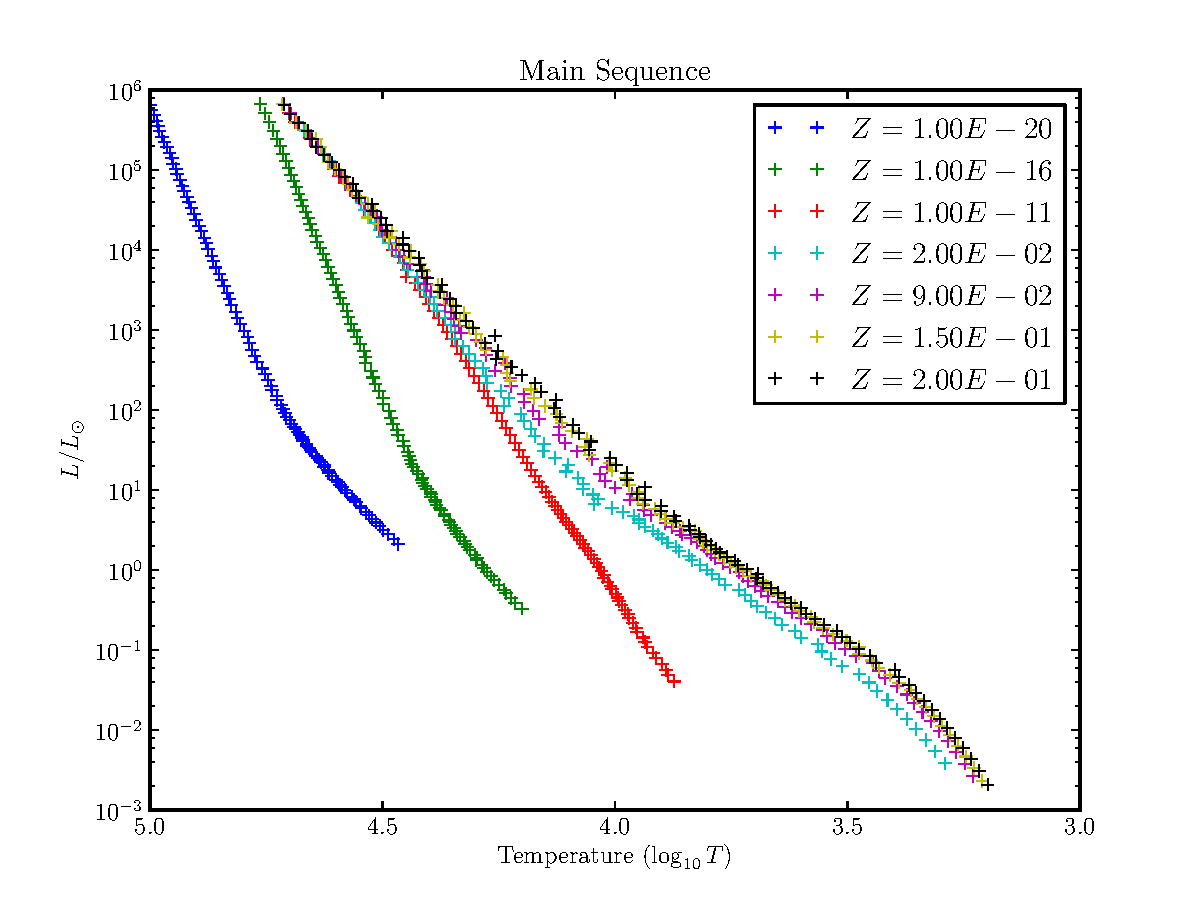
\includegraphics[width=\textwidth]{figures/ms.pdf}
            \caption{Main Sequence with varying metallicity.}
            \label{fig:ms}
        \end{figure}
    \end{center}
    \begin{center}
        \begin{figure}[H]
            \begin{subfigure}{.5\textwidth}
                \centering
                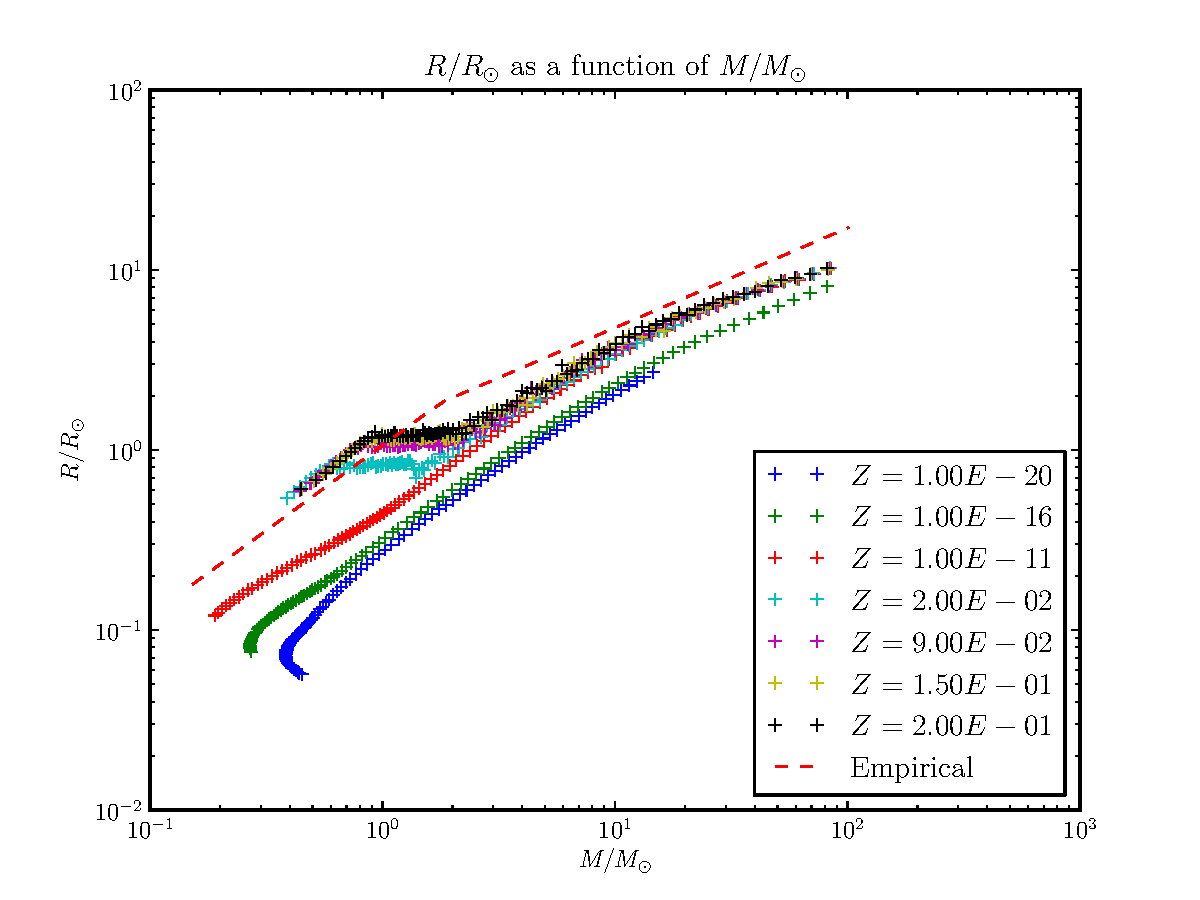
\includegraphics[width=1.1\textwidth]{figures/RvM.pdf}
                \caption{Radius and mass relationship with varying metallicity.}
                \label{fig:RvM}
            \end{subfigure}
            \begin{subfigure}{.5\textwidth}
                \centering
                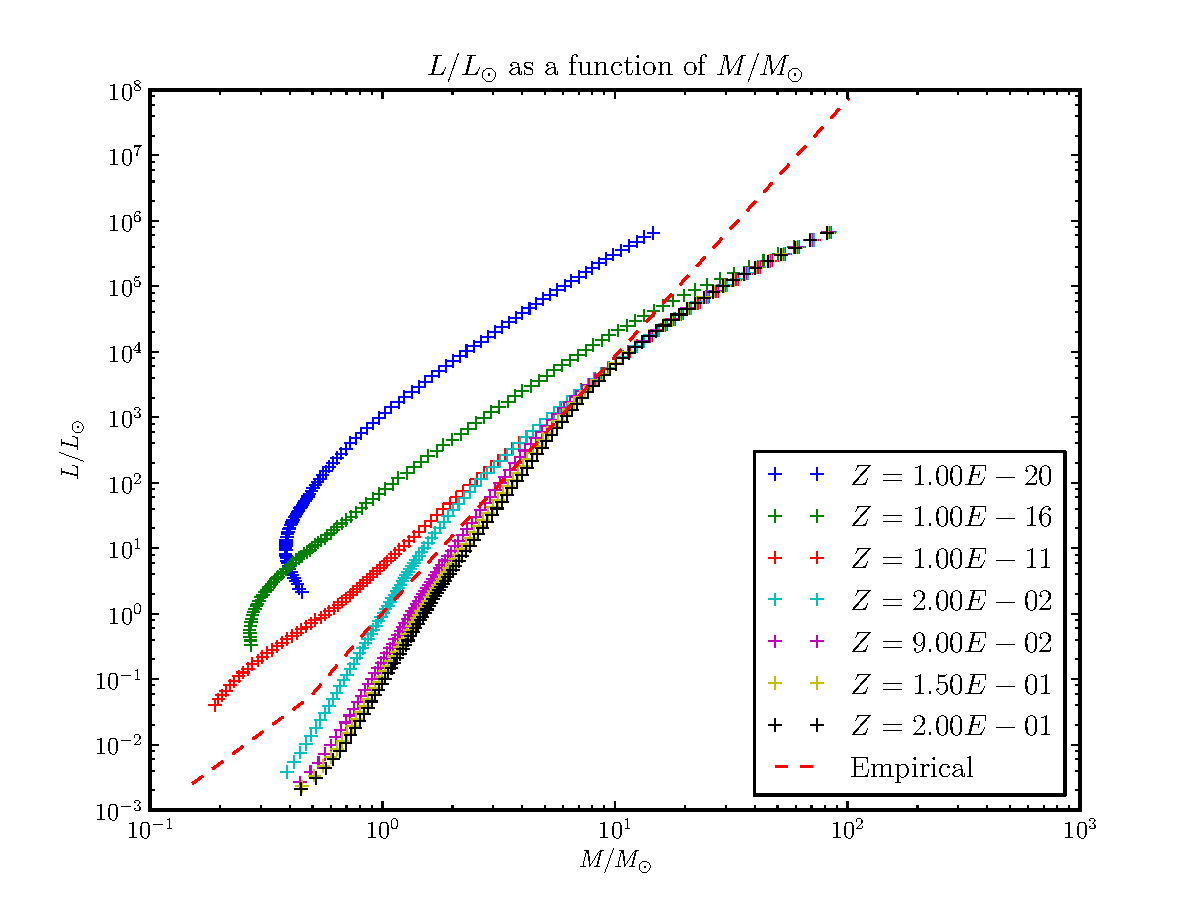
\includegraphics[width=1.1\textwidth]{figures/LvM.pdf}
                \caption{Luminosity and radius relationship with varying metallicity.}
                \label{fig:LvM}
            \end{subfigure}
        \end{figure}
    \end{center}
    \section{Suggested Improvements}
    There are numerous improves and further work that can be done using this model for stellar structure. \\

    Firstly, as discussed in section \ref{sec:opacity} the limit as $Z$ approaches $0$ is both non-physical and not supported by the opacity model \eqref{eq:kh}. These extreme composition environments require more careful treatment of equations involving composition. Therefore, it is recommended more complicated opacity models should be introduced. Additionally, a model for ionization levels should be incorporated instead treating all material as being ionized. This would involved the Saha equation and other statistical mechanics techniques. Moreover, the composition of a star is not radially fixed. Heavier nuclei are synthesized in the core of a star where energy production occurs. Including the production of heavy nuclei in the core would put lower bounds on the metallicity mass fraction $Z$ in the center of the star. \\

    Secondly, this entire project took the hydrogen mass fraction to be a constant equal to the solar value. More realistically, an increasing $Z$ would decrease both $X$ and $Y$ in a stratified way. Work should be done to determine if modifying $Y$ instead of $Z$ has any appreciable affect on mass sequence plots. \\

    Finally, more work needs to be done in order to determine the mechanism behind the ``hooks'' found in low metallicity, low mass stars in figures \ref{fig:LvM} and \ref{fig:RvM}. This behavior seems to indicate that the physics of very low temperature stars with low metallicities are counter-intuitive and would be an excellent avenue for further study.
    \bibliography{report}{}
    \bibliographystyle{plain}
\end{document}